\documentclass[10pt]{beamer}

\usetheme[progressbar=frametitle]{metropolis}
\usepackage{appendixnumberbeamer}

\usepackage{booktabs}
\usepackage[scale=2]{ccicons}

\usepackage{pgfplots}
\usepgfplotslibrary{dateplot}

\usepackage{braket} %ket vectors
\usepackage[font=footnotesize,labelfont=bf]{caption}
\usepackage{parskip} %automatic paragraphing
\usepackage{color}
\usepackage{dsfont}%identity operator
\usepackage{mathrsfs}
\usepackage{xspace}
\usepackage{xcolor}
\usepackage{amsmath,amsfonts} %for gathering equations
\usepackage{siunitx} %for SI units
\usepackage{pgfplots} %for plotting
%\usepackage{multimedia}
\usepackage{media9}
\usepackage{xcolor,colortbl}
%\usepackage{fancyvrb}
%\usepackage{array}
\newcolumntype{C}[1]{>{\centering\let\newline\\\arraybackslash\hspace{0pt}}m{#1}}
\definecolor{darkyellow}{HTML}{FFB600}
\definecolor{emerald}{HTML}{32936F}
\definecolor{red1}{HTML}{FF0000}
\definecolor{red2}{HTML}{B20000}
\definecolor{red3}{HTML}{7F0000}
\definecolor{red4}{HTML}{FF3217}
\definecolor{red5}{HTML}{FF0D48}
\definecolor{blue1}{HTML}{0000FF}
\definecolor{blue2}{HTML}{0000B5}
\definecolor{blue3}{HTML}{000080}
\definecolor{blue4}{HTML}{3C00FF}
\definecolor{blue5}{HTML}{3C5DFF}
\definecolor{inputblue1}{HTML}{0000CC}
\definecolor{inputmixblue2}{HTML}{002DF7}
\definecolor{inputmixblue3}{HTML}{3C8BFF}
\definecolor{inputmixblue4}{HTML}{6730A8}
\definecolor{inputred1}{HTML}{970000}
\definecolor{inputmixred2}{HTML}{DF3100}
\definecolor{inputmixred3}{HTML}{C43335}
\definecolor{inputmixred4}{HTML}{DE366C}

\usepackage{filecontents} %for data loading
\begin{filecontents}{datax.dat}
0.06941, 28, 0.44096, 30, 0.15165, 25
0.04389, 146, 0.32707, 132,0.10722, 109
0.02823, 3622, 0.08416, 3478, 0.02086, 2997
0.01008, 17838, 0.005179, 17566, 0.01494, 14721
0.00165, 89130,0.0015799, 88216, 0.003327, 74009
0.00156, 444646, 0.0015601, 439060, 0.001578, 370813
%previous 3rd row: 0.04951, 728, 0.224107, 642, 0.020864, 601
\end{filecontents}
\begin{filecontents}{scatterplot.dat}
x y class
0.1 0.4 b
0.4 0.2 r
\end{filecontents}
\begin{filecontents}{scattered_example2.dat}
3.45, 643, 589, 3.76, 3.52
2.78, 558, 512, 2.87, 2.91
2.52, 583, 503, 2.54, 2.4
3.67, 685, 602, 3.83, 3.47
3.24, 592, 538, 3.29, 3.47
2.1, 562, 486, 2.64, 2.37 
\end{filecontents}

\usepackage[cal=zapfc,calscaled=.96]{mathalfa}

\newcommand{\themename}{\textbf{\textsc{metropolis}}\xspace}

\title{Quantum-enhanced machine learning: Implementing a quantum $k$-nearest neighbour algorithm}
\subtitle{Bachelor thesis defense \newline 19. January 2017}
%\subtitle{19. January 2017}
%\date{\today}
\date{}
\author{Mark Fingerhuth}
\institute{Maastricht Science Programme, Maastricht University, The Netherlands \newline Thesis work at the Centre for Quantum Technology, UKZN, South Africa \newline

\begin{minipage}[c]{0.49\textwidth}

\includegraphics[scale=0.3]{UM_logo.eps}
\end{minipage}%%%
%\hspace{0.5cm}
\begin{minipage}[c]{0.49\textwidth}
\flushright

\includegraphics[scale=0.35]{logo.jpeg} 
\end{minipage}
}
% \titlegraphic{\hfill
\includegraphics[height=1.5cm]{logo.pdf}}

\begin{document}

\maketitle

\begin{frame}{Table of contents}
  %\setbeamertemplate{section in toc}[sections numbered]
  %\tableofcontents %[hideallsubsections]
  \begin{enumerate}
  \item Introduction
  \item Machine Learning
  \item Quantum Computing
  \item Quantum-enhanced Machine Learning
  \item Results: Amplitude-based quantum $k$-nearest neighbour algorithm
  \item Outlook
  \item Conclusion
  \end{enumerate}
\end{frame}


\section{Introduction}

{
\setbeamertemplate{frame footer}{\tiny{\textsuperscript{1}Bishop, C. M. (2006). Pattern recognition. Machine Learning, 128 .\newline \textsuperscript{2}Bekkerman, R., Bilenko, M., \& Langford, J. (2011). Scaling up machine learning: Parallel and distributed
approaches. Cambridge University Press.}}
\begin{frame}[fragile]{Enhancing machine learning with quantum mechanics}

\begin{minipage}[c]{0.45\textwidth}
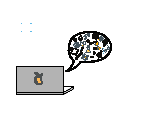
\includegraphics[scale=3.5]{Vectors/laptop_ml.eps}
\newline
\textbf{Machine learning}\\
Enable computers to\\
learn from data
\end{minipage}%%
\hspace{0.5cm}
\begin{minipage}[c]{0.49\textwidth}
\flushright
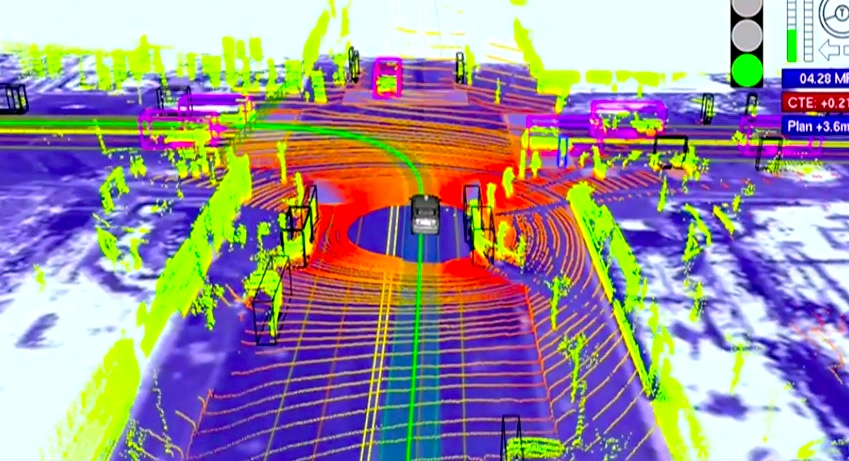
\includegraphics[scale=0.09]{google_car.jpeg}
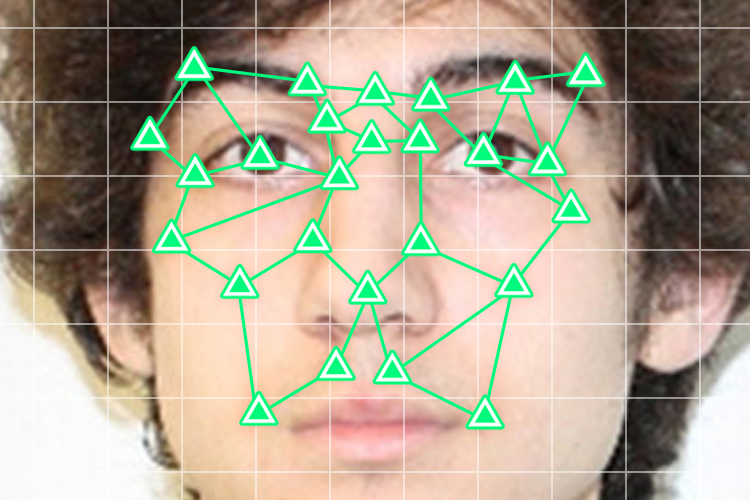
\includegraphics[scale=0.55]{facial_recognition.jpg}\\
\vspace{-0.2cm}
\tiny{Source: IEEE Spectrum}
\normalsize
\vspace{0.5cm}
\flushleft
\begin{itemize}	 
%Approximately 2.5 quintillion (${10}^{18}$) bytes of digital data are created every day\textsuperscript{1}
	\item ML algorithms often involve\textsuperscript{1}
	\begin{itemize}
	\item solving large systems of linear equations
	\item inverting large matrices
	\item distance computations
	\end{itemize}
	\item Performing these computations on large data
sets gets increasingly difficult\textsuperscript{2}
\end{itemize}
\end{minipage}


\end{frame}
}

{
\setbeamertemplate{frame footer}{}
\begin{frame}[fragile]{Quantum Machine Learning}

\begin{enumerate}
\item ML involves manipulation of large vectors and matrices
\item Quantum mechanics is about vectors $\in$ complex Hilbert spaces
\item Quantum computers are performing linear operations on qubits
\end{enumerate}
\hspace{3mm}$\rightarrow$ Hence, we can manipulate large vectors in parallel on quantum\\ \hspace{8mm}computers\\
\vspace{3mm}
\centering{\textcolor{orange}{So can we use QC to improve classical ML algorithms??}}
\vspace{3mm}
\begin{itemize}
\item Classical ML is a very practical topic\\
\item BUT, QML has been of almost entirely theoretical nature
\end{itemize}
\end{frame}
}

{
\setbeamertemplate{frame footer}{\tiny{\textsuperscript{1}}}
\begin{frame}[fragile]{Enhancing machine learning with quantum mechanics}
\hspace{-0.7cm}
\begin{minipage}[c]{0.59\textwidth}
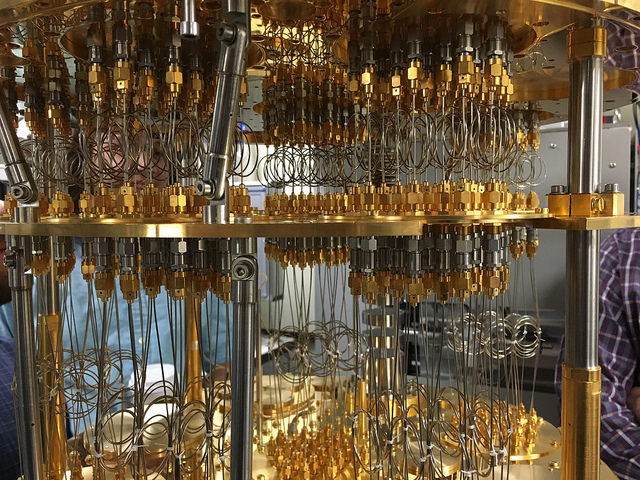
\includegraphics[scale=0.12]{ibm-quantum-computer.jpg}
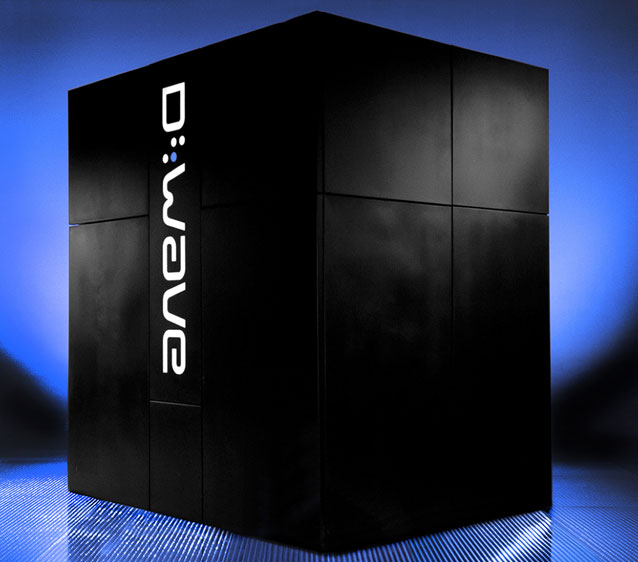
\includegraphics[scale=0.12]{dwave.jpg}
\tiny{Sources: DWave, IBM}
\normalsize
\begin{itemize}
\item Quantum mechanics is about vectors in complex Hilbert spaces
\item Quantum computers are performing linear operations on qubits
\item Many-qubit systems are described by large vectors that can be manipulated in parallel on quantum computers
\item Machine learning involves manipulation of large vectors and matrices
\end{itemize}
\end{minipage}%%
\hspace{0.3cm}
\begin{minipage}[c]{0.39\textwidth}
\vspace{2.8cm}
\centering
\hspace{-1cm}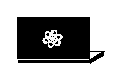
\includegraphics[scale=2.2]{Vectors/laptop_q.eps}
\flushleft
\textbf{Quantum computing}\\
Build computer hardware based on quantum physics
\end{minipage}

\end{frame}
}

{
\setbeamertemplate{frame footer}{\tiny{\textsuperscript{1}}}
\begin{frame}[fragile]{Enhancing machine learning with quantum mechanics}

\begin{minipage}[c]{0.59\textwidth}
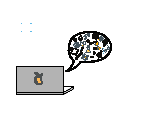
\includegraphics[scale=3.5]{Vectors/laptop_ml.eps}
\newline
\textbf{Machine learning}\\
Enable computers to\\
learn from data
\end{minipage}%%
\begin{minipage}[c]{0.39\textwidth}
\vspace{2.8cm}
\centering
\hspace{-1cm}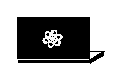
\includegraphics[scale=2.2]{Vectors/laptop_q.eps}
\flushleft
\textbf{Quantum computing}\\
Build computer hardware based on quantum physics
\end{minipage}

\end{frame}
}

{
\setbeamertemplate{frame footer}{\tiny{\textsuperscript{1}}}
\begin{frame}[fragile]{Enhancing machine learning with quantum mechanics}

\begin{figure}
\centering
\hspace{2cm}
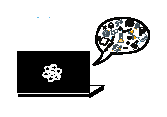
\includegraphics[scale=3]{Vectors/laptop_qml.eps}
\end{figure}
\centering
\textbf{Quantum-enhanced machine learning}\\
Enable quantum computers to learn from data\\
faster than classical computers

\end{frame}
}


\section{\protect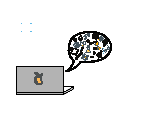
\includegraphics[scale=3.5]{Vectors/laptop_ml.eps}\newline Machine Learning
}

{
\setbeamertemplate{frame footer}{\tiny{\textsuperscript{1}}}
\begin{frame}[fragile]{Supervised machine learning}

\begin{table}
\begin{tabular}{| C{0.45cm} | C{1cm} |C{1.4cm} |}
    \toprule
      ID & Colour & Class label\\
      \midrule
       1 & \cellcolor{red1} & red \\\midrule
       2 &\cellcolor{red2} & red \\\midrule
       3 & \cellcolor{red3} & red \\\midrule\midrule
       4 & \cellcolor{blue1} & blue \\\midrule
       5 & \cellcolor{blue2} & blue \\\midrule
       6 & \cellcolor{blue3} & blue \\
      \bottomrule
    \end{tabular}
    \caption{Example training dataset.}
\end{table}

\begin{equation}
f(x) = o\, .
\end{equation}
\begin{equation}
f(\colorbox{red2}{colour}) = red\, .
\end{equation}
\begin{itemize}
\item Labelled training dataset $\rightarrow$ supervision!
\end{itemize}

\end{frame}
}

{
\setbeamertemplate{frame footer}{\tiny{\textsuperscript{1}}}
\begin{frame}[fragile]{Supervised machine learning}

\begin{table}
\centering
    \begin{tabular}{| C{0.45cm} | C{1cm} |C{1.4cm}|}
    \toprule
      ID & Colour & Class label \\
      \midrule
       1 & \cellcolor{inputred1} &  ?\\\midrule
      
       2 & \cellcolor{inputblue1} & ? \\
      \bottomrule
    \end{tabular}
    \caption{Example input dataset.}
\end{table}

The machine learning algorithm should approximate the function $f$ such that it can predict the output $o$ for a new unknown input $\tilde{x}$:
\begin{equation}
f(\tilde{x}) = ?\, .
\end{equation}

\end{frame}
}



{
\setbeamertemplate{frame footer}{\tiny{\textsuperscript{1}}}
\begin{frame}[fragile]{Classical $k$-nearest neighbour}

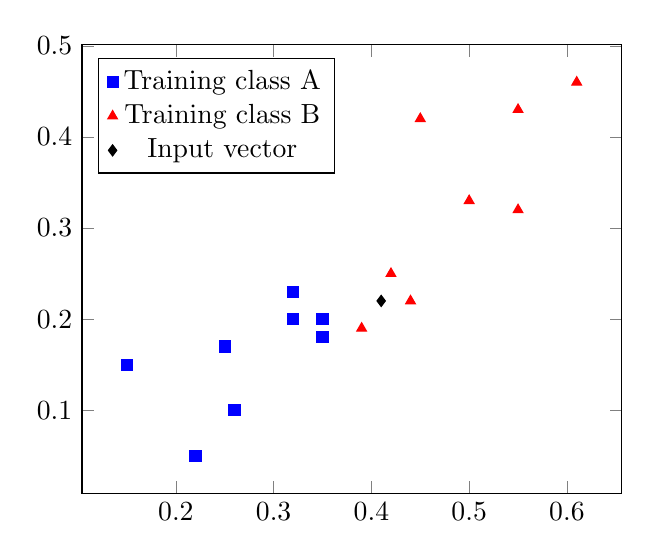
\begin{tikzpicture} \begin{axis}[legend pos=north west, scatter/classes={ a={mark=square*,blue}, b={mark=triangle*,red}, c={mark=diamond*,draw=black}}] \addplot[scatter,only marks, scatter src=explicit symbolic] table[meta=label] {
x y label
0.15 0.15 a
0.25 0.17 a
0.26 0.1 a
0.22 0.05 a

0.35 0.18 a
0.32 0.2 a
0.32 0.23 a
0.35 0.2 a
0.42 0.25 b
0.44 0.22 b
0.39 0.19 b

0.45 0.42 b
0.55 0.32 b

0.61 0.46 b
0.5 0.33 b
0.55 0.43 b
0.41 0.22 c
};
\addlegendentry{Training class A}
\addlegendentry{Training class B}
\addlegendentry{Input vector}
\end{axis}
\end{tikzpicture}



\end{frame}
}

{
\setbeamertemplate{frame footer}{\tiny{\textsuperscript{1}}}
\begin{frame}[fragile]{Classical $k$-nearest neighbour}

\begin{minipage}[c]{0.49\textwidth}
\centering
$k = 3$\\
\vspace{0.5cm}
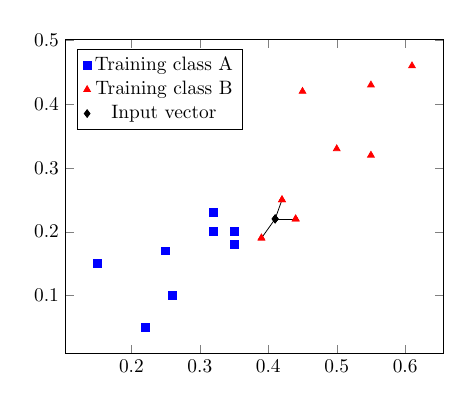
\begin{tikzpicture}[scale=0.7]
\begin{axis}[legend pos=north west,
			scatter/classes={
			a={mark=square*,blue}, 												b={mark=triangle*,red}, 											c={mark=diamond*,draw=black}}]
			\addplot[scatter,only marks, scatter src=explicit symbolic]
table[meta=label] {
x y label
0.15 0.15 a
0.25 0.17 a
0.26 0.1 a
0.22 0.05 a

0.35 0.18 a
0.32 0.2 a
0.32 0.23 a
0.35 0.2 a
0.42 0.25 b
0.44 0.22 b
0.39 0.19 b

0.45 0.42 b
0.55 0.32 b

0.61 0.46 b
0.5 0.33 b
0.55 0.43 b
0.41 0.22 c
};
\addplot[scatter, scatter src=explicit symbolic]
table[meta=label] {
x y label
%0.35 0.18 a
%0.32 0.2 a
%0.32 0.23 a
%0.35 0.2 a
0.42 0.25 b
%0.44 0.22 b
%0.39 0.19 b
0.41 0.22 c
};
\addplot[scatter, scatter src=explicit symbolic]
table[meta=label] {
x y label
%0.35 0.18 a
%0.32 0.2 a
%0.32 0.23 a
%0.35 0.2 a
%0.42 0.25 b
0.44 0.22 b
%0.39 0.19 b
0.41 0.22 c
};
\addplot[scatter, scatter src=explicit symbolic]
table[meta=label] {
x y label
%0.35 0.18 a
%0.32 0.2 a
%0.32 0.23 a
%0.35 0.2 a
%0.42 0.25 b
%0.44 0.22 b
0.39 0.19 b
0.41 0.22 c
};
\addlegendentry{Training class A}
\addlegendentry{Training class B}
\addlegendentry{Input vector}
\end{axis}
\end{tikzpicture}
\end{minipage}%%%
\begin{minipage}[c]{0.49\textwidth}
\centering
$k = 7$\\
\vspace{0.5cm}
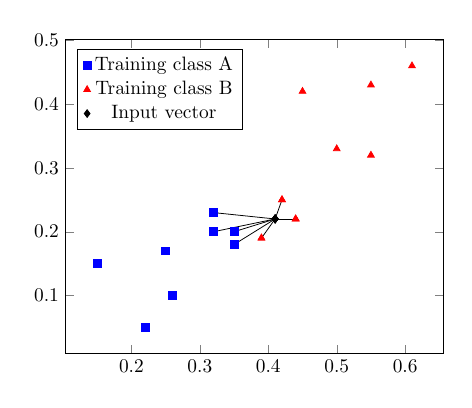
\begin{tikzpicture}[scale=0.7]
\begin{axis}[legend pos=north west,
			scatter/classes={
			a={mark=square*,blue}, 												b={mark=triangle*,red}, 											c={mark=diamond*,draw=black}}]
			\addplot[scatter,only marks, scatter src=explicit symbolic]
table[meta=label] {
x y label
0.15 0.15 a
0.25 0.17 a
0.26 0.1 a
0.22 0.05 a

0.35 0.18 a
0.32 0.2 a
0.32 0.23 a
0.35 0.2 a
0.42 0.25 b
0.44 0.22 b
0.39 0.19 b

0.45 0.42 b
0.55 0.32 b

0.61 0.46 b
0.5 0.33 b
0.55 0.43 b
0.41 0.22 c
};
\addplot[scatter, scatter src=explicit symbolic]
table[meta=label] {
x y label
0.35 0.18 a
%0.32 0.2 a
%0.32 0.23 a
%0.35 0.2 a
%0.42 0.25 b
%0.44 0.22 b
%0.39 0.19 b
0.41 0.22 c
};
\addplot[scatter, scatter src=explicit symbolic]
table[meta=label] {
x y label
%0.35 0.18 a
0.32 0.2 a
%0.32 0.23 a
%0.35 0.2 a
%0.42 0.25 b
%0.44 0.22 b
%0.39 0.19 b
0.41 0.22 c
};
\addplot[scatter, scatter src=explicit symbolic]
table[meta=label] {
x y label
%0.35 0.18 a
%0.32 0.2 a
0.32 0.23 a
%0.35 0.2 a
%0.42 0.25 b
%0.44 0.22 b
%0.39 0.19 b
0.41 0.22 c
};
\addplot[scatter, scatter src=explicit symbolic]
table[meta=label] {
x y label
%0.35 0.18 a
%0.32 0.2 a
%0.32 0.23 a
0.35 0.2 a
%0.42 0.25 b
%0.44 0.22 b
%0.39 0.19 b
0.41 0.22 c
};
\addplot[scatter, scatter src=explicit symbolic]
table[meta=label] {
x y label
%0.35 0.18 a
%0.32 0.2 a
%0.32 0.23 a
%0.35 0.2 a
0.42 0.25 b
%0.44 0.22 b
%0.39 0.19 b
0.41 0.22 c
};
\addplot[scatter, scatter src=explicit symbolic]
table[meta=label] {
x y label
%0.35 0.18 a
%0.32 0.2 a
%0.32 0.23 a
%0.35 0.2 a
%0.42 0.25 b
0.44 0.22 b
%0.39 0.19 b
0.41 0.22 c
};
\addplot[scatter, scatter src=explicit symbolic]
table[meta=label] {
x y label
%0.35 0.18 a
%0.32 0.2 a
%0.32 0.23 a
%0.35 0.2 a
%0.42 0.25 b
%0.44 0.22 b
0.39 0.19 b
0.41 0.22 c
};
\addlegendentry{Training class A}
\addlegendentry{Training class B}
\addlegendentry{Input vector}
\end{axis}
\end{tikzpicture}
\end{minipage}
\end{frame}
}

{
\setbeamertemplate{frame footer}{\tiny{\textsuperscript{1}}}
\begin{frame}[fragile]{Classical $k$-nearest neighbour}

Explain the kNN!

\end{frame}
}


\section{\protect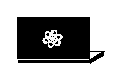
\includegraphics[scale=2.4]{Vectors/laptop_q.eps}\newline Quantum Computing}

{
\setbeamertemplate{frame footer}{\tiny{\textsuperscript{1}}}
\begin{frame}[fragile]{Classical vs. quantum bits (qubits)}

PICTURE OF MOSFET

Classical bit:
\begin{itemize}
\item Usually implemented through MOSFETs
\item 2 definite states ($0$,$1$)
\item Can be either $0$ OR $1$
\end{itemize}

\end{frame}
}

{
\setbeamertemplate{frame footer}{\tiny{\textsuperscript{1}Reprinted from RF Wireless World, n.d., Retrieved December 23, 2016, from \url{http://www.rfwireless-world.com/Terminology/Difference-between-Bit-and-Qubit.html}. Copyright 2012 by RF Wireless World.}}
\begin{frame}[fragile]{Classical vs. quantum bits (qubits)}

Quantum bit (qubit):
\begin{itemize}
\item Can be $0$ OR $1$
\item But it can also be $0$ AND $1$ $\rightarrow$ quantum superposition
\end{itemize}

\begin{figure}
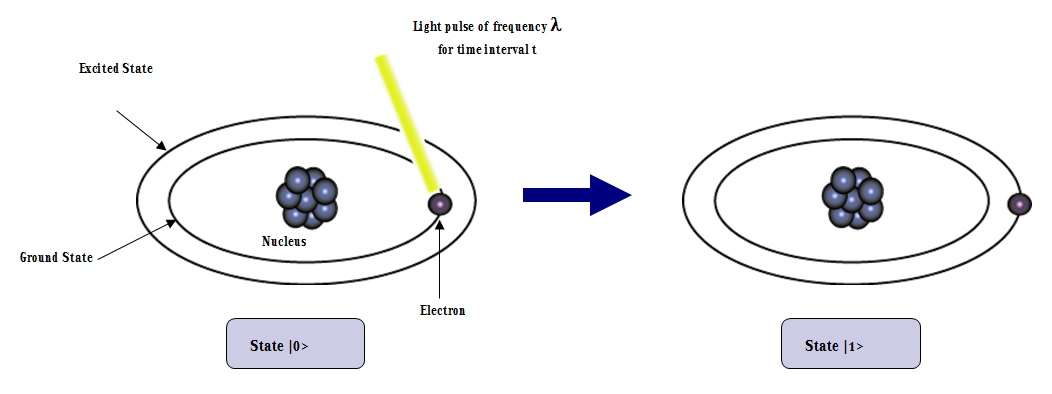
\includegraphics[scale=0.3]{qubitimplementation.jpeg}
\caption{Example of a physical qubit.\textsuperscript{1}}
\end{figure}

%introduce ket vectors \& superposition
%show vector representation of a qubit
\end{frame}
}

{
\setbeamertemplate{frame footer}{\tiny{}}
\begin{frame}[fragile]{Qubits}

Mathematically, a qubit state is expressed as:
\begin{equation}
\label{equ:simplequbit}
\ket{\psi} = \alpha \ket{0} + \beta \ket{1}\, ,
\end{equation}
where $\alpha, \beta \in \mathbb{C}$ and they are called amplitudes.

$\ket{0}$ and $\ket{1}$ can be represented as the 2-D vectors:
\begin{equation}
\ket{0} \doteq  \begin{pmatrix}1\\0\end{pmatrix} \quad \mathrm{and} \quad \ket{1} \doteq \begin{pmatrix}0\\1\end{pmatrix}\, .
\end{equation}

Substituting into Eq.~\ref{equ:simplequbit} yields the vector representation of $\ket{\psi}$:
\begin{equation}
\ket{\psi} \doteq \alpha \begin{pmatrix} 1\\0 \end{pmatrix} + \beta \begin{pmatrix}0\\1 \end{pmatrix} = \begin{pmatrix}\alpha\\\beta\end{pmatrix}\, .
\end{equation}

%introduce ket vectors \& superposition
%show vector representation of a qubit
\end{frame}
}

{
\setbeamertemplate{frame footer}{\tiny{\textsuperscript{1}Reprinted from Wikipedia, n.d., Retrieved September 7, 2016, from \url{https://en.wikipedia.org/wiki/Bloch_Sphere}. Copyright 2012 by Glosser.ca. Reprinted with permission.}}
\begin{frame}[fragile]{The Bloch sphere}

\begin{minipage}[c]{.5\textwidth}
		%\centering
		\hspace{2mm}
       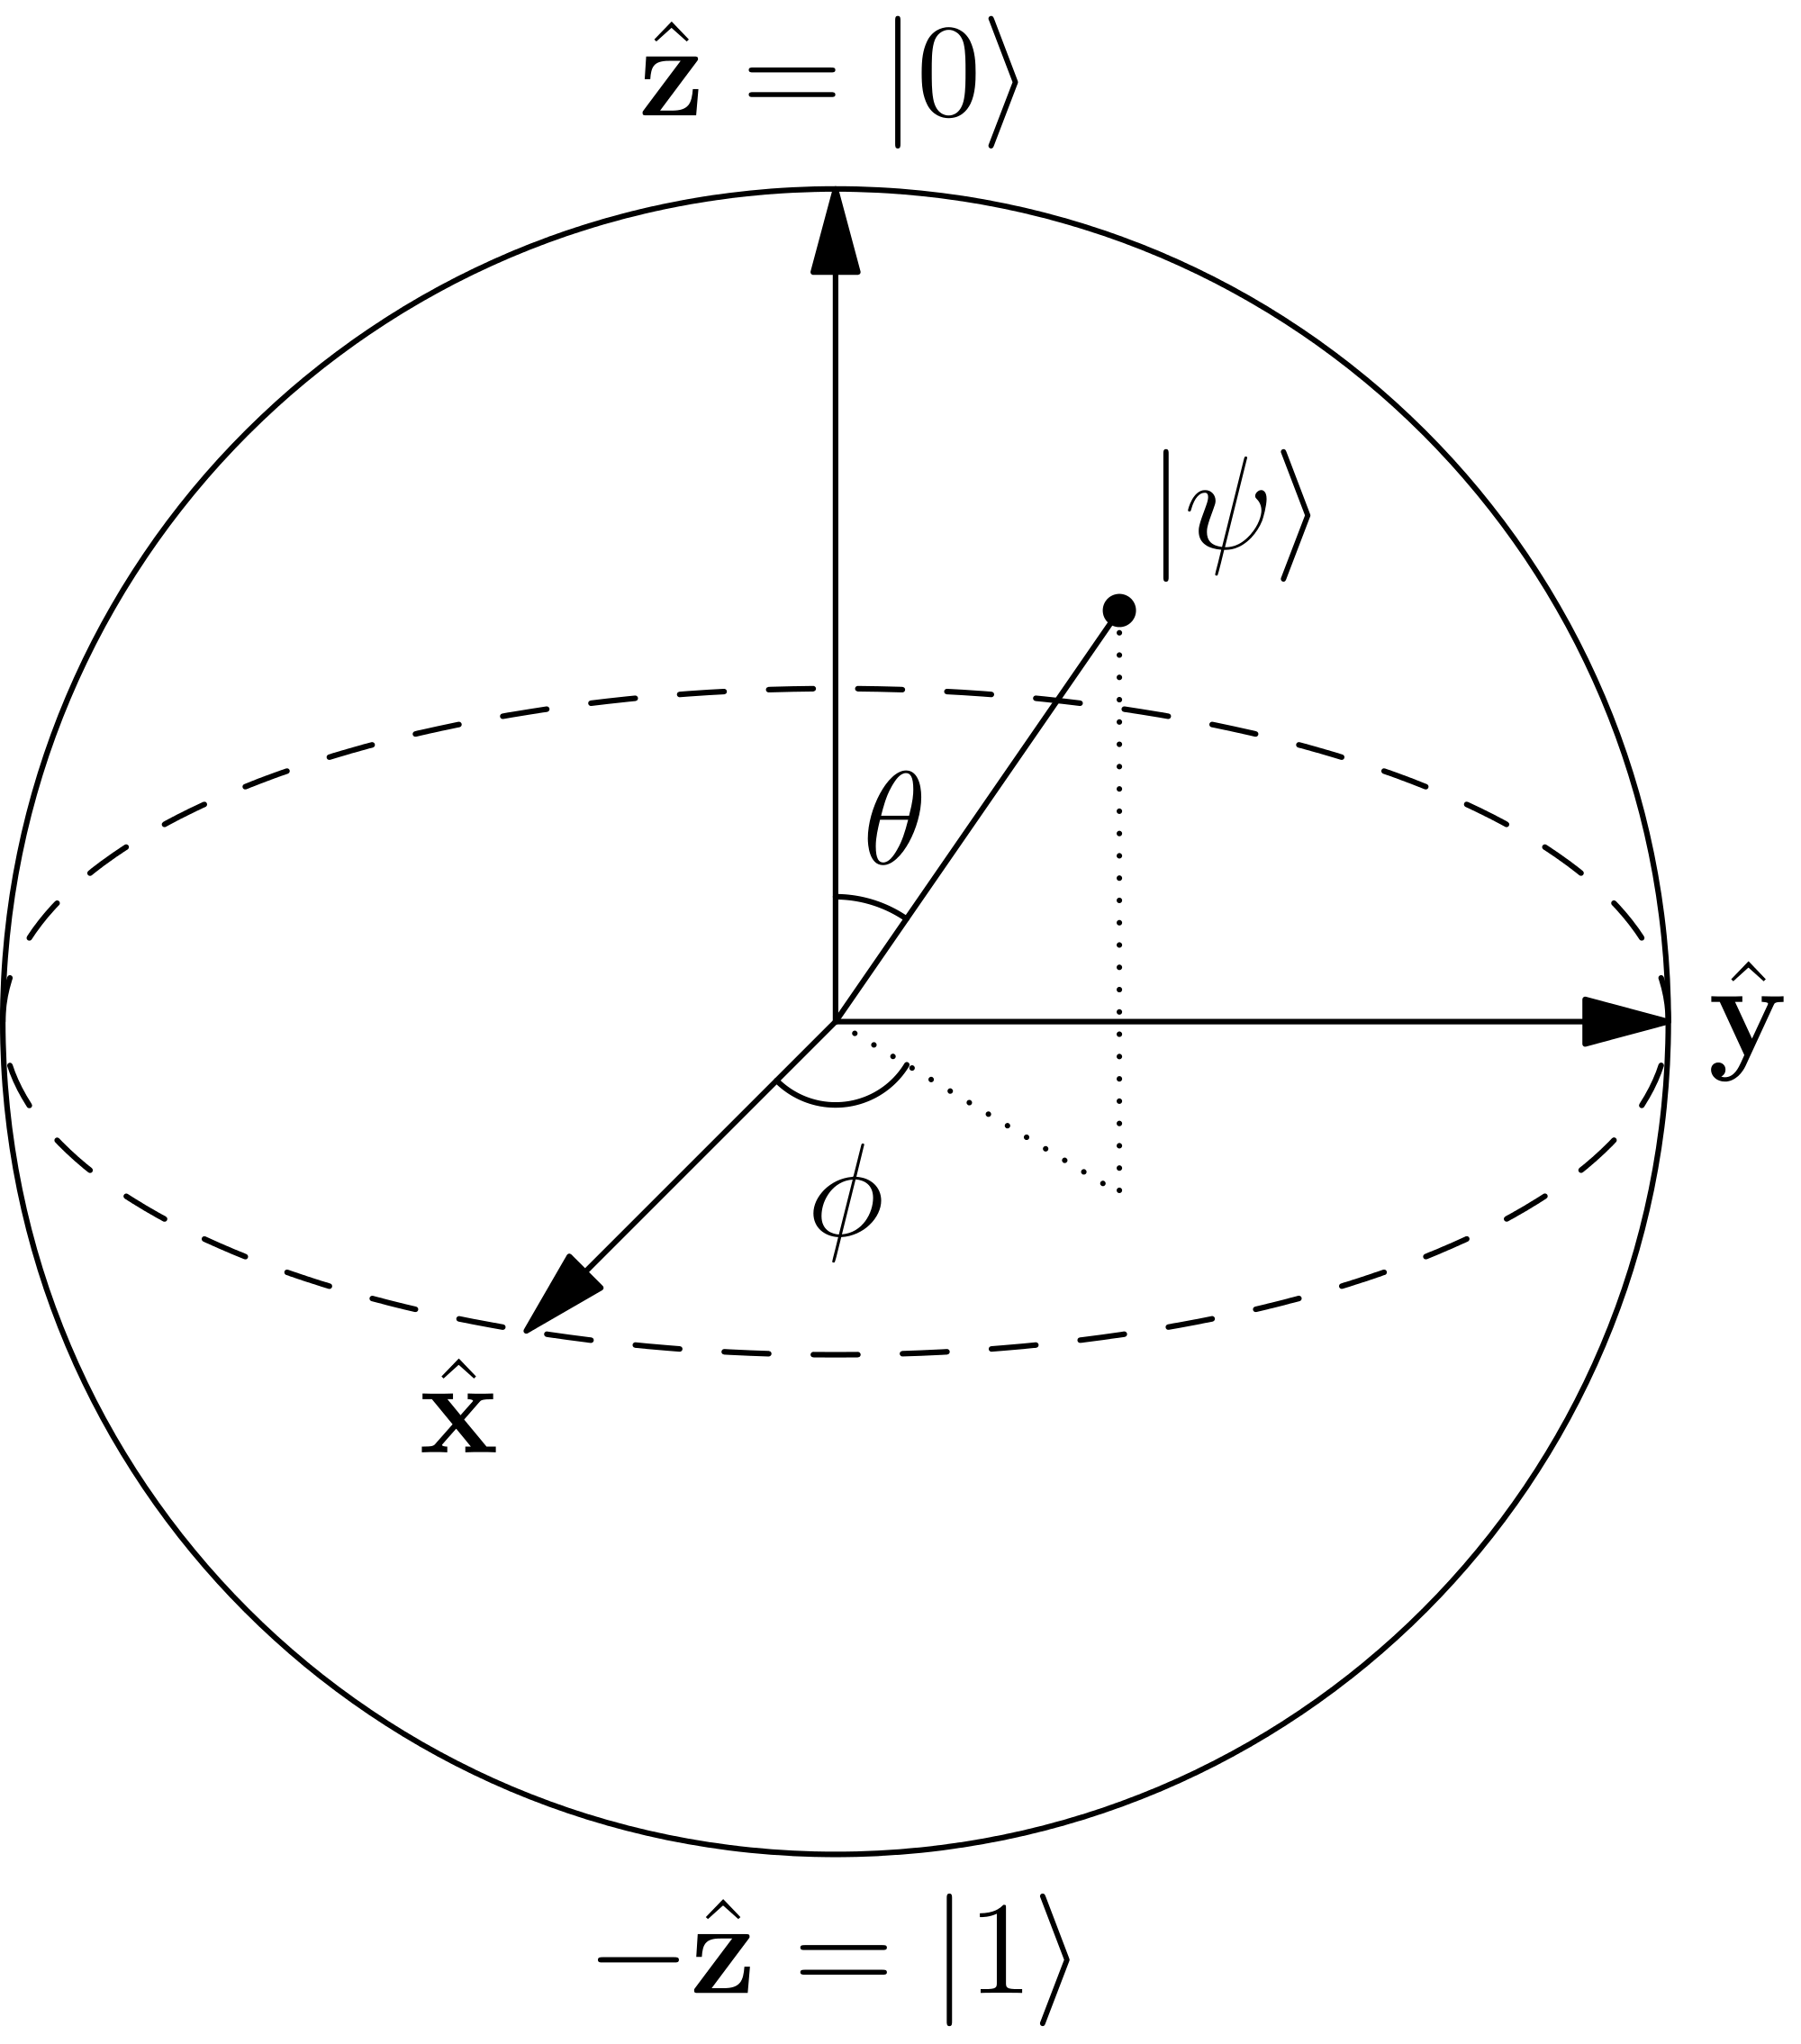
\includegraphics[width=0.8\textwidth]{blochsphere.png}
       \captionsetup{justification=raggedright, singlelinecheck=false}
       \captionof{figure}{\footnotesize{Arbitrary two-dimensional qubit $\ket{\psi}$ visualized on the Bloch sphere\textsuperscript{1}} }
\end{minipage}%%%%%
\begin{minipage}[c][][b]{.5\textwidth}
Most general form of a 2-D qubit:
\begin{equation}
\label{equ: blochqubit}
\ket{\psi} = \alpha \ket{0} + \beta \ket{1}\, ,
\end{equation}
where $\alpha,\beta \in \mathbb{C}$.\\
\\
Can also be visualized in spherical polar coords on the unit or Bloch sphere as follows: 

\begin{equation}
\label{equ: blochqubit}
\ket{\psi} = \cos\frac{\theta}{2} \ket{0} + e^{i \phi} \sin\frac{\theta}{2} \ket{1}\, ,
\end{equation}
where $0 \leq \theta \leq \pi$ and $0 \leq \phi \leq 2\pi$
\null
\par\xdef\tpd{\the\prevdepth}
\end{minipage}

\end{frame}
}

{
\setbeamertemplate{frame footer}{\tiny{}}
\begin{frame}[fragile]{Three random bits vs. three qubits}

Mathematically, a qubit state is expressed as:
\begin{equation}
\label{equ:simplequbit}
\ket{\psi} = \alpha \ket{0} + \beta \ket{1}\, ,
\end{equation}
where $\alpha, \beta \in \mathbb{C}$ and they are called amplitudes.

$\ket{0}$ and $\ket{1}$ can be represented as the 2-D vectors:
\begin{equation}
\ket{0} \doteq  \begin{pmatrix}1\\0\end{pmatrix} \quad \mathrm{and} \quad \ket{1} \doteq \begin{pmatrix}0\\1\end{pmatrix}\, .
\end{equation}

Substituting into Eq.~\ref{equ:simplequbit} yields the vector representation of $\ket{\psi}$:
\begin{equation}
\ket{\psi} \doteq \alpha \begin{pmatrix} 1\\0 \end{pmatrix} + \beta \begin{pmatrix}0\\1 \end{pmatrix} = \begin{pmatrix}\alpha\\\beta\end{pmatrix}\, .
\end{equation}

%introduce ket vectors \& superposition
%show vector representation of a qubit
\end{frame}
}

{
\setbeamertemplate{frame footer}{\tiny{\textsuperscript{1}}}
\begin{frame}[fragile]{Quantum gates}

\begin{equation}
\label{equ:unitarytransformation}
U \ket{\psi} \doteq \begin{pmatrix}
 a & b \\ 
 c & d
 \end{pmatrix} \begin{pmatrix} \alpha\\ \beta \end{pmatrix}= \begin{pmatrix} a\alpha+b\beta\\c\alpha+d\beta\end{pmatrix}\, .
\end{equation}
show matrix representation
show matrix vector multiplication??
Show two simple examples (Hadamard and X gate?)

\end{frame}
}


\section*{\protect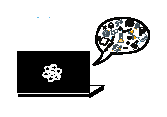
\includegraphics[scale=2.4]{Vectors/laptop_qml.eps}\newline Quantum-enhanced Machine Learning}

{
\setbeamertemplate{frame footer}{\tiny{\textsuperscript{1}}}
\begin{frame}[fragile]{Encoding classical data into qubits}

%\movie[width=5cm,height=3.8cm,poster,autostart]{}{interference.mp4}
%\includemedia[
%  label=vidA,
%  addresource=interference.mp4,
%  activate=pageopen,
%  width=5cm, height=3.8cm,
%  flashvars={
%     source=interference.mp4
%    &loop=true
%  }
%]{}{VPlayer.swf}

%\mediabutton[
%  mediacommand=vidA:playPause,
%]{\fbox{Play/Pause}}
%\begin{figure}[ht]
%\includemovie[poster,text={\small(Loading Video...)}]{6cm}{4cm}{interference.mp4}
%\end{figure}
There are two fundamentally different ways for state preparation:

\begin{alertblock}{Data encoded into qubits}
%speed-up not very clear since the \# of qubits increases linearly with the \# of classical bits
k-dimensional probability vector requires $4k$ classical bits which are encoded one-to-one into $4k$ qubits, e.g.\\
\vspace{2mm}
$\begin{pmatrix}
 \textcolor{blue}{0.6} \\ 
 \textcolor{emerald}{0.4}
 \end{pmatrix}*10 \rightarrow \begin{pmatrix}
 \textcolor{blue}{6} \\ 
 \textcolor{emerald}{4}
 \end{pmatrix} \rightarrow \begin{pmatrix}
 \textcolor{blue}{0110} \\ 
 \textcolor{emerald}{0100}
 \end{pmatrix} \rightarrow n=\textcolor{blue}{0110}\textcolor{emerald}{0100} \rightarrow \ket{n} = \ket{\textcolor{blue}{0110}\textcolor{emerald}{0100}}$\\
%\textbf{Only slight speed up possible}
\end{alertblock}
\vspace{3mm}
\begin{alertblock}{\textcolor{gray}{Data encoded into amplitudes}}
\textcolor{gray}{k-dimensional probability vector is encoded into $log_{2}(k)$ qubits, e.g.\\ 
\vspace{2mm}
$\begin{pmatrix}
 0.6 \\ 
 0.4
 \end{pmatrix} \quad \rightarrow \quad \ket{n} = \sqrt{0.6}\ket{0}+\sqrt{0.4}\ket{1}$\\
%\textbf{Possibility of exponential speed up}
}
\end{alertblock}


\end{frame}
}

{
\setbeamertemplate{frame footer}{\tiny{\textsuperscript{1}}}
\begin{frame}[fragile]{Encoding classical data into amplitudes}
There are two fundamentally different ways for state preparation:

\begin{alertblock}{\textcolor{gray}{Data encoded into qubits}}
%speed-up not very clear since the \# of qubits increases linearly with the \# of classical bits
\textcolor{gray}{k-dimensional probability vector requires $4k$ classical bits which are encoded one-to-one into $4k$ qubits, e.g.\\
\vspace{2mm}
$\begin{pmatrix}
 0.6 \\ 
 0.4
 \end{pmatrix}*10 \rightarrow \begin{pmatrix}
 6 \\ 
 4
 \end{pmatrix} \rightarrow \begin{pmatrix}
 0110 \\ 
 0100
 \end{pmatrix} \rightarrow n=01100100 \rightarrow \ket{n} = \ket{01100100}$\\
%\textbf{Only slight speed up possible}
}
\end{alertblock}  
\vspace{3mm}
\begin{alertblock}{Data encoded into amplitudes}
k-dimensional probability vector is encoded into $log_{2}(k)$ qubits, e.g.\\ 
\vspace{2mm}
$\begin{pmatrix}
 \textcolor{blue}{0.6} \\ 
 \textcolor{emerald}{0.4}
 \end{pmatrix} \quad \rightarrow \quad \ket{n} = \sqrt{\textcolor{blue}{0.6}}\ket{0}+\sqrt{\textcolor{emerald}{0.4}}\ket{1}$\\
%\textbf{Possibility of exponential speed up}
\end{alertblock}

\end{frame}
}

{
\setbeamertemplate{frame footer}{\tiny{\textsuperscript{1}}}
\begin{frame}[fragile]{Calculating distances with interference}


\end{frame}
}


\section{Results: Qubit-based kNN algorithm}

{
\setbeamertemplate{frame footer}{\tiny{\textsuperscript{1}}}
\begin{frame}[fragile]{}




\end{frame}
}


\section{Results: Amplitude-based kNN algorithm}

{
\setbeamertemplate{frame footer}{\tiny{\textsuperscript{1}}}
\begin{frame}[fragile]{}
efesafefesf



\end{frame}
}

{
\setbeamertemplate{frame footer}{\tiny{\textsuperscript{1}Reprinted from Wikipedia, n.d., Retrieved September 7, 2016, from \url{https://en.wikipedia.org/wiki/Bloch_Sphere}. Copyright 2012 by Glosser.ca. Reprinted with permission.}}
\begin{frame}[fragile]{Quantum Computing \& Qubits}

\begin{minipage}[c]{.5\textwidth}
		%\centering
		\hspace{2mm}
       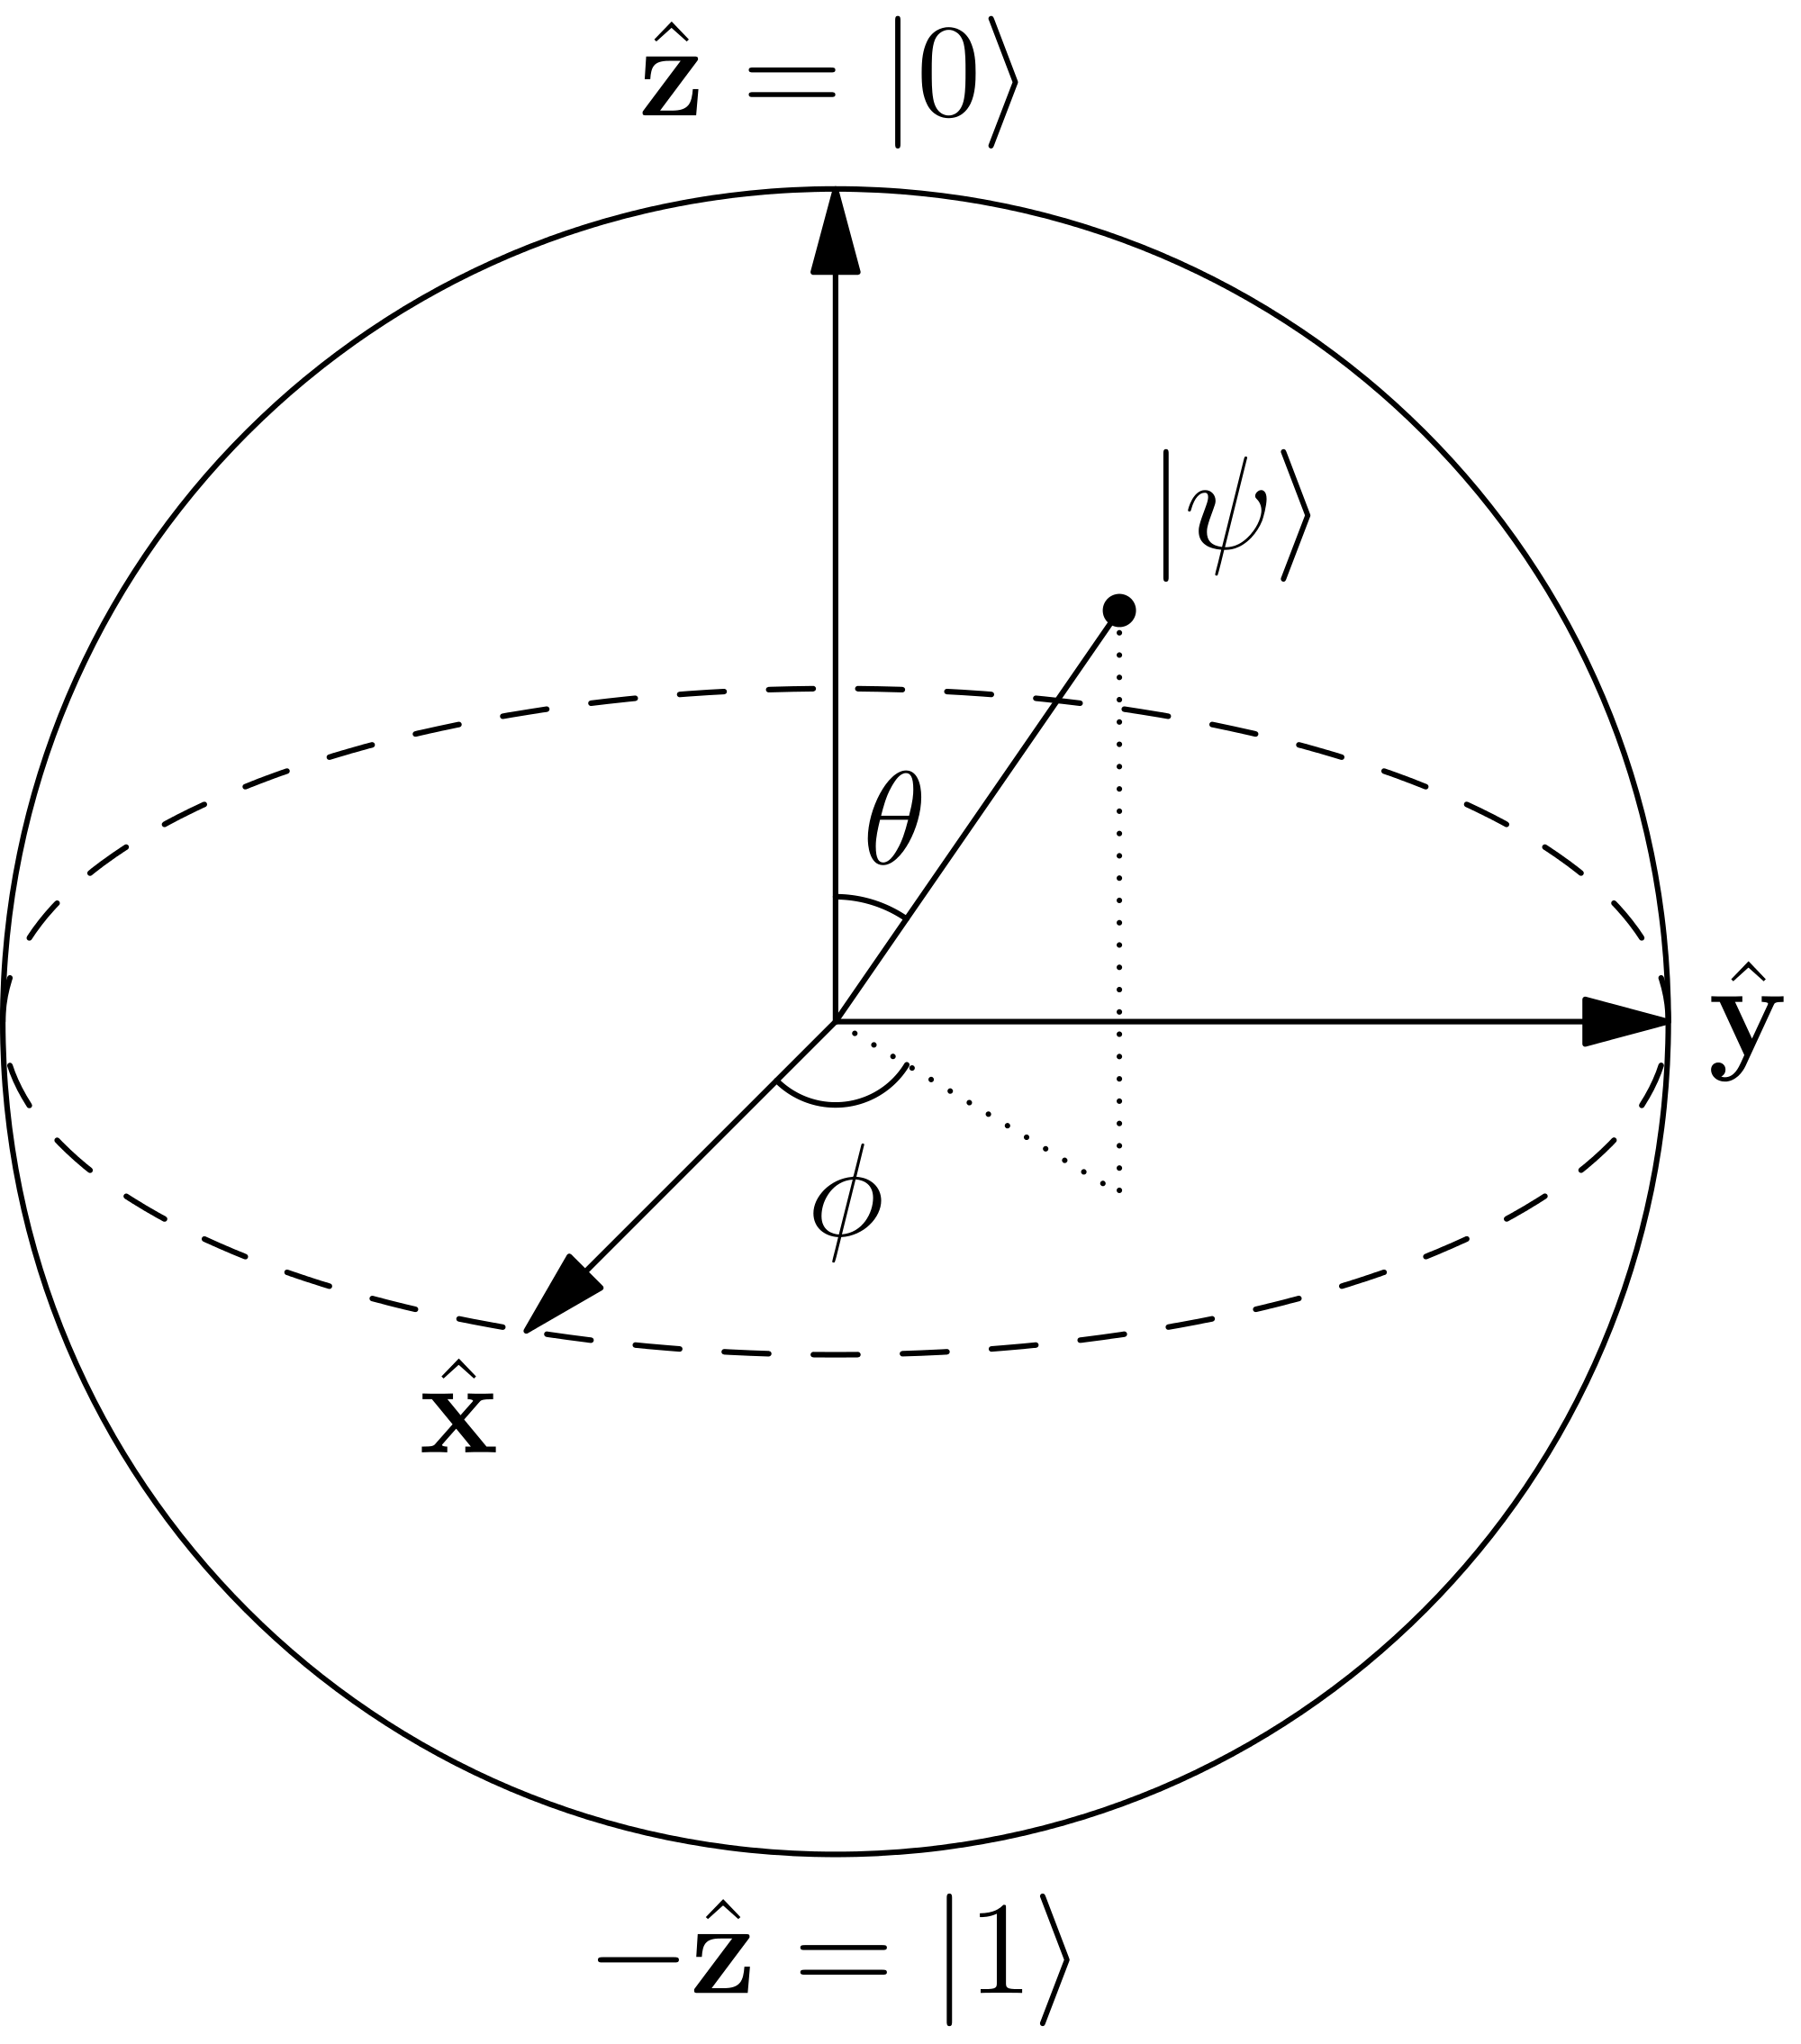
\includegraphics[width=0.8\textwidth]{blochsphere.png}
       \captionsetup{justification=raggedright, singlelinecheck=false}
       \captionof{figure}{\footnotesize{Arbitrary two-dimensional qubit $\ket{\psi}$ visualized on the Bloch sphere\textsuperscript{1}} }
\end{minipage}%%%%%
\begin{minipage}[c][][b]{.5\textwidth}
Most general form of a 2-D qubit:
\begin{equation}
\label{equ: blochqubit}
\ket{q} = \alpha \ket{0} + \beta \ket{1}
\end{equation}
where $\alpha,\beta \in \mathbb{C}$.\\
\\
Can also be visualized in spherical polar coords on the unit or Bloch sphere as follows: 

\begin{equation}
\label{equ: blochqubit}
\ket{q} = \cos\frac{\theta}{2} \ket{0} + e^{i \phi} \sin\frac{\theta}{2} \ket{1}
\end{equation}
where $0 \leq \theta \leq \pi$ and $0 \leq \phi \leq 2\pi$
\null
\par\xdef\tpd{\the\prevdepth}
\end{minipage}


\end{frame}
}

{
\setbeamertemplate{frame footer}{\tiny{\textsuperscript{1}IBM. (2016). What is big data? https://www-01.ibm.com/software/data/bigdata/what-is-big
-data.html. (Accessed: 2016-09-08) \newline
\textsuperscript{2}Bekkerman, R., Bilenko, M., \& Langford, J. (2011). Scaling up machine learning: Parallel and distributed
approaches. Cambridge University Press.}}
\begin{frame}[fragile]{Machine Learning}
   
\begin{itemize}
	\item Approximately 2.5 quintillion (${10}^{18}$) bytes of digital data are created every day\textsuperscript{1}
	\item Need for advanced algorithms that can make sense of data content, retrieve patterns and reveal correlations $\rightarrow$ Machine learning (ML) 
	\item ML algorithms often involve
	\begin{itemize}
	\item solving large systems of linear equations
	\item inverting large matrices
	\item distance computations
	\end{itemize}
	\item Performing these computations on large data
sets gets increasingly difficult\textsuperscript{2}

%when i.e. $\mathcal{O}(input size)$ or $\mathcal{O}(input size^{k})$ for some constant k\textsuperscript{2}
%essentially manipulations on big vectors and matrices

\end{itemize}

\end{frame}
}

{
\setbeamertemplate{frame footer}{}
\begin{frame}[fragile]{Quantum Machine Learning}

\begin{enumerate}
\item ML involves manipulation of large vectors and matrices
\item Quantum mechanics is about vectors $\in$ complex Hilbert spaces
\item Quantum computers are performing linear operations on qubits
\end{enumerate}
\hspace{3mm}$\rightarrow$ Hence, we can manipulate large vectors in parallel on quantum\\ \hspace{8mm}computers\\
\vspace{3mm}
\centering{\textcolor{orange}{So can we use QC to improve classical ML algorithms??}}
\vspace{3mm}
\begin{itemize}
\item Classical ML is a very practical topic\\
\item BUT, QML has been of almost entirely theoretical nature
\end{itemize}
\end{frame}
}

{
\setbeamertemplate{frame footer}{}
\begin{frame}[fragile]{Quantum data encoding}
 
There are two fundamentally different ways for state preparation:

\begin{alertblock}{Data encoded into qubits}
%speed-up not very clear since the \# of qubits increases linearly with the \# of classical bits
k-dimensional probability vector requires $4k$ classical bits which are encoded one-to-one into $4k$ qubits, e.g.\\
\vspace{2mm}
$\begin{pmatrix}
 \textcolor{blue}{0.6} \\ 
 \textcolor{emerald}{0.4}
 \end{pmatrix}*10 \rightarrow \begin{pmatrix}
 \textcolor{blue}{6} \\ 
 \textcolor{emerald}{4}
 \end{pmatrix} \rightarrow \begin{pmatrix}
 \textcolor{blue}{0110} \\ 
 \textcolor{emerald}{0100}
 \end{pmatrix} \rightarrow n=\textcolor{blue}{0110}\textcolor{emerald}{0100} \rightarrow \ket{n} = \ket{\textcolor{blue}{0110}\textcolor{emerald}{0100}}$\\
%\textbf{Only slight speed up possible}
\end{alertblock}
\vspace{3mm}
\begin{alertblock}{\textcolor{gray}{Data encoded into amplitudes}}
\textcolor{gray}{k-dimensional probability vector is encoded into $log_{2}(k)$ qubits, e.g.\\ 
\vspace{2mm}
$\begin{pmatrix}
 0.6 \\ 
 0.4
 \end{pmatrix} \quad \rightarrow \quad \ket{n} = \sqrt{0.6}\ket{0}+\sqrt{0.4}\ket{1}$\\
%\textbf{Possibility of exponential speed up}
}
\end{alertblock}

\end{frame}
}

{
\setbeamertemplate{frame footer}{}
\begin{frame}[fragile]{Quantum data encoding}
 
There are two fundamentally different ways for state preparation:

\begin{alertblock}{\textcolor{gray}{Data encoded into qubits}}
%speed-up not very clear since the \# of qubits increases linearly with the \# of classical bits
\textcolor{gray}{k-dimensional probability vector requires $4k$ classical bits which are encoded one-to-one into $4k$ qubits, e.g.\\
\vspace{2mm}
$\begin{pmatrix}
 0.6 \\ 
 0.4
 \end{pmatrix}*10 \rightarrow \begin{pmatrix}
 6 \\ 
 4
 \end{pmatrix} \rightarrow \begin{pmatrix}
 0110 \\ 
 0100
 \end{pmatrix} \rightarrow n=01100100 \rightarrow \ket{n} = \ket{01100100}$\\
%\textbf{Only slight speed up possible}
}
\end{alertblock}  
\vspace{3mm}
\begin{alertblock}{Data encoded into amplitudes}
k-dimensional probability vector is encoded into $log_{2}(k)$ qubits, e.g.\\ 
\vspace{2mm}
$\begin{pmatrix}
 \textcolor{blue}{0.6} \\ 
 \textcolor{emerald}{0.4}
 \end{pmatrix} \quad \rightarrow \quad \ket{n} = \sqrt{\textcolor{blue}{0.6}}\ket{0}+\sqrt{\textcolor{emerald}{0.4}}\ket{1}$\\
%\textbf{Possibility of exponential speed up}
\end{alertblock}


\end{frame}
}

{
\setbeamertemplate{frame footer}{\tiny{\textsuperscript{1}Reprinted from GitHub, Burton de Wilde, Retrieved September 13, 2016, from http://bdewilde.github.io/blog/
blogger/2012/10/26/classification-of-hand-written-digits-3/. Copyright 2012 by Burton de Wilde. Reprinted with
permission.}}
\begin{frame}[fragile]{Classical k-nearest neighbour}
 

\centering{
- kNN is a non-parametric classifier\\
- $k$ is a positive integer, usually chosen small}

\begin{minipage}[t]{.35\textwidth}
Given training data set:\\
${D}_{T}$ = ${v}_{0}, {v}_{1},..,{v}_{10}$ \\
$v_{i} \in$ \{$A$, $B$\}

\end{minipage}%%%
\begin{minipage}[t]{.65\textwidth}
Given a new vector $\tilde{x}$ (red star):\\
- consider $k$ nearest neighbours\\
- classify $\tilde{x}$, based on majority vote, as $A$ or $B$
\end{minipage}

\begin{figure}
       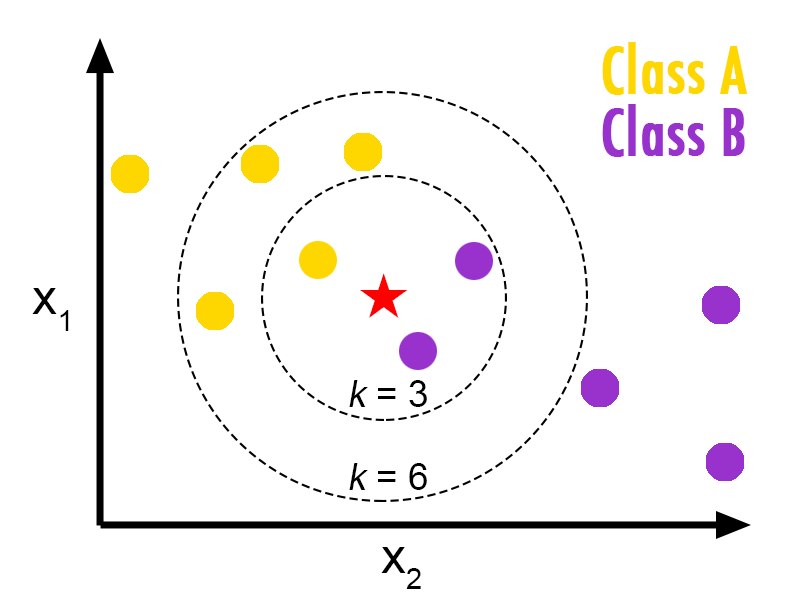
\includegraphics[width=0.5\textwidth]{knn-concept.png}
      \caption{\footnotesize{Visualization of a kNN classifier\footnotemark[1]}}
\end{figure}
 
\end{frame}
}


%\section{Amplitude-based kNN algorithm}
{
\setbeamertemplate{frame footer}{\vspace{-2mm}\tiny{Maria Schuld (2016), unpublished}}
\begin{frame}{The algorithm}

\begin{equation}
\frac{1}{\sqrt{2M}}\sum_{m=1}^{M} (\textcolor{emerald}{\ket{0}}\ket{\textcolor{red}{\Psi_{\tilde{x}} (\star)}}+\textcolor{emerald}{\ket{1}}\ket{\textcolor{darkyellow}{\Psi}_{\textcolor{purple}{x^{m}}}})\ket{y^{m}(\textcolor{darkyellow}{A} \ or \ \textcolor{purple}{B})}\ket{m}
\end{equation}
where
\begin{equation}
\ket{\textcolor{red}{\Psi_{\tilde{x}} (\star)}} = \sum_{i=1}^{N} \textcolor{red}{\tilde{x}_i}\ket{i} \quad \quad
\ket{\textcolor{darkyellow}{\Psi}_{\textcolor{purple}{x^{m}}}}	 = \sum_{i=1}^{N} \textcolor{darkyellow}{x}\textcolor{purple}{_i^m} \ket{i} 
\end{equation}

\begin{equation}
e.g. \quad \begin{pmatrix}
 \textcolor{blue}{0.6} \\ 
 \textcolor{emerald}{0.4}
 \end{pmatrix} \quad \rightarrow \quad \ket{n} =  \sqrt{\textcolor{blue}{0.6}}\ket{0}+\sqrt{\textcolor{emerald}{0.4}}\ket{1}
\end{equation}

\begin{figure}
       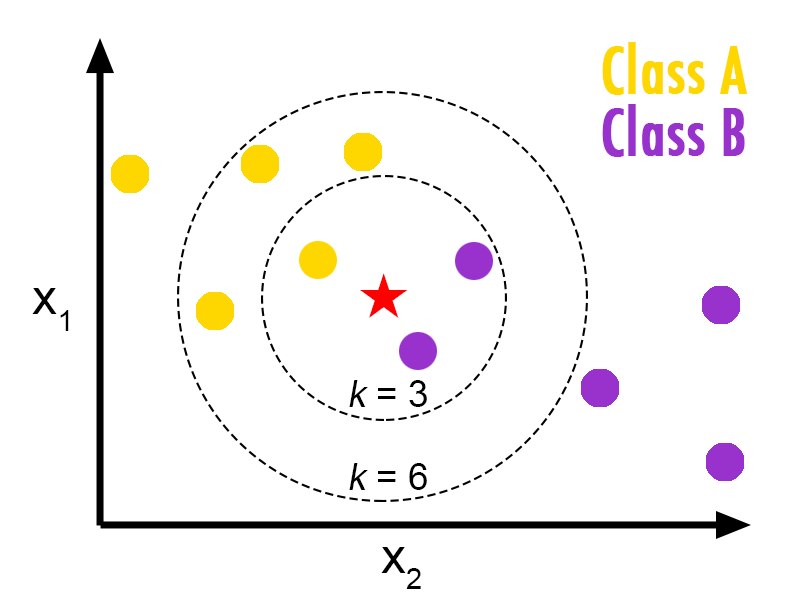
\includegraphics[scale=.25]{knn-concept.png}
      \caption{\footnotesize{Visualization of a kNN classifier\footnotemark[1]}}
\end{figure}

\end{frame}
}

{
\setbeamertemplate{frame footer}{\vspace{-2mm}\tiny{Maria Schuld (2016), unpublished}}
\begin{frame}{The algorithm}

Applying the \textbf{Hadamard gate} interferes the input and the training vectors:

\begin{equation}
\frac{1}{2\sqrt{M}}\sum_{m=1}^{M} (\textcolor{emerald}{\ket{0}}[\ket{\textcolor{red}{\Psi_{\tilde{x}}}}+\ket{\textcolor{darkyellow}{\Psi}_{\textcolor{purple}{x^{m}}}}]+\textcolor{emerald}{\ket{1}}[\ket{\textcolor{red}{\Psi_{\tilde{x}}}}-\ket{\textcolor{darkyellow}{\Psi}_{\textcolor{purple}{x^{m}}}}])\ket{y^{m}(\textcolor{darkyellow}{A} \ or \ \textcolor{purple}{B})}\ket{m}
\end{equation}

$\rightarrow$ Perform \textbf{conditional measurement} on ancilla qubit.\\
Successful if $\ket{0}$ state is measured.
\end{frame}
}

{
\setbeamertemplate{frame footer}{\vspace{-2mm}\tiny{Maria Schuld (2016), unpublished}}
\begin{frame}{The algorithm}

After successful conditional measurement, the state is proportional to
\begin{equation}
\frac{1}{2\sqrt{M}}\sum_{m=1}^{M} \sum_{i=1}^{N} (\textcolor{red}{\tilde{x}_i}+\textcolor{darkyellow}{x}\textcolor{purple}{_i^m})\ket{0}\ket{i}\ket{y^{m}(\textcolor{darkyellow}{A} \ or \ \textcolor{purple}{B})}\ket{m}
\end{equation}

Probability to measure class B:
\begin{equation}
p(\ket{y^m} = \ket{1(\textcolor{purple}{B})})= \sum_{m \mid y^m=1(\textcolor{purple}{B})} 1 - \frac{1}{4M} \mid \textcolor{red}{\tilde{x}} - \textcolor{purple}{x^m} \mid ^2
\end{equation}
	\metroset{block=fill}
	\begin{alertblock}{Overall algorithmic complexity}
	\centering
	$\mathcal{O}(\frac{1}{p_{acc}})$ where $p_{acc}$ is the probability of measuring ancilla in the $\ket{0}$ state
	\end{alertblock}
\end{frame}
}


{
\setbeamertemplate{frame footer}{}
\begin{frame}{Simple binary classification case}

\begin{minipage}[c]{.4\textwidth}
		%\centering
		\hspace{-7mm}
       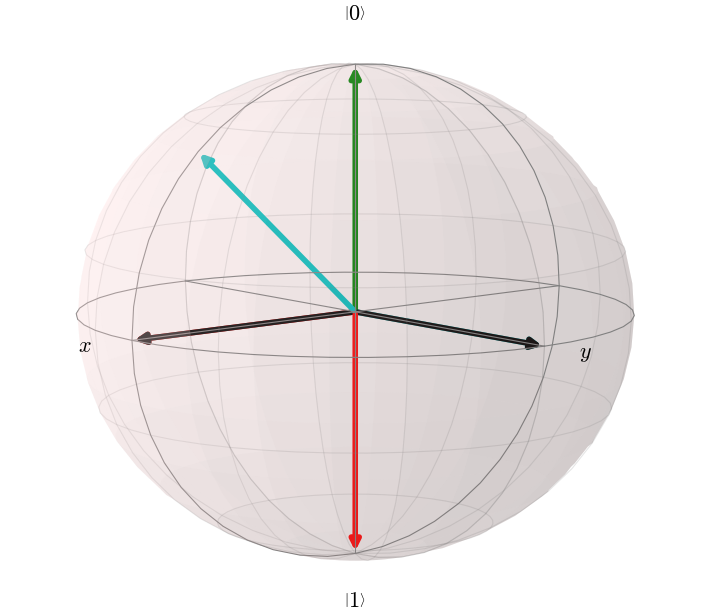
\includegraphics[width=1.1\textwidth]{bloch3over4.png}
       \captionsetup{justification=raggedright, singlelinecheck=false}
       \captionof{figure}{\footnotesize{Simple binary classification problem of a quantum state} }
\end{minipage}%%%%
\begin{minipage}[c][][b]{.6\textwidth}
\scriptsize{
\begin{equation}
\frac{1}{\sqrt{2M}}\sum_{m=1}^{M} (\textcolor{emerald}{\ket{0}}\ket{\textcolor{red}{\Psi_{\tilde{x}} (\star)}}+\textcolor{emerald}{\ket{1}}\ket{\textcolor{darkyellow}{\Psi}_{\textcolor{purple}{x^{m}}}})\ket{y^{m}(\textcolor{darkyellow}{A} \ or \ \textcolor{purple}{B})}\ket{m}
\end{equation}}
Procedure to load the input vector $\tilde{x}$:
\begin{equation}
\ket{\Psi_0} = \frac{1}{2}\sum_{m=1}^{2} (\textcolor{emerald}{\ket{0}}\ket{0}+\textcolor{emerald}{\ket{1}}\ket{0})\ket{y^{m}}\ket{m}
\end{equation}
Apply controlled rotation $_0^1CR_y(\frac{\pi}{4})$ s.t.
\begin{equation}
_0^1CR_y(\frac{\pi}{4})\ket{\Psi_0} = \ket{\Psi_1} = \frac{1}{2}\sum_{m=1}^{2} (\textcolor{emerald}{\ket{0}}\ket{0}+\textcolor{emerald}{\ket{1}}\ket{\textcolor{red}{\Psi_{\tilde{x}}}})\ket{y^{m}}\ket{m}
\end{equation}
Flip the ancilla qubit in the first register
\begin{equation}
(X\otimes\mathds{1}\otimes\mathds{1}\otimes\mathds{1})\ket{\Psi_1} = \ket{\Psi_2} = \frac{1}{2}\sum_{m=1}^{2} (\textcolor{emerald}{\ket{0}}\ket{\textcolor{red}{\Psi_{\tilde{x}}}}+\textcolor{emerald}{\ket{1}}\ket{0})\ket{y^{m}}\ket{m}
\end{equation}
\null
\par\xdef\tpd{\the\prevdepth}
\end{minipage}

	%\metroset{block=fill}
	%\begin{alertblock}{Algorithmic complexity}
	%\centering
	%$\mathcal{O}(\frac{1}{p_{acc}})$
	%\end{alertblock}

\end{frame}
}

{
\setbeamertemplate{frame footer}{}
\begin{frame}{Implementation with IBM's quantum computer}

\begin{figure}
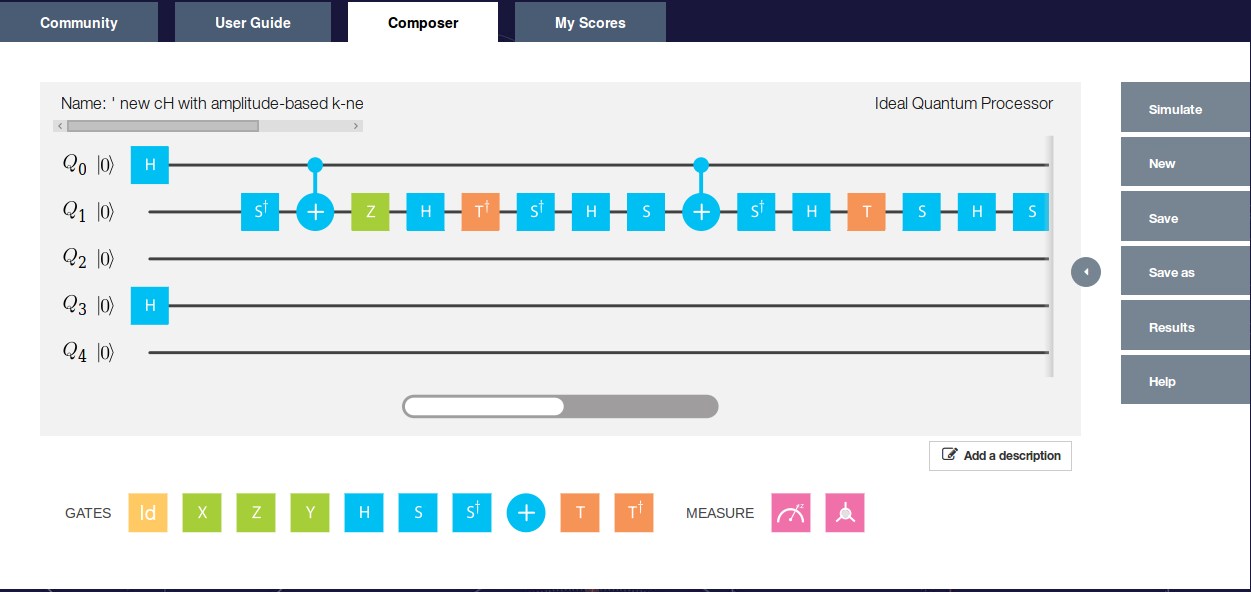
\includegraphics[height=0.5\textwidth]{IBMamplitudecomposer.png}
       \caption{\footnotesize{IBM's quantum composer} }
\end{figure}
\vspace{-5mm}
\begin{minipage}[t]{.5\textwidth}
\begin{itemize}
\item Accessible to the public
\item Allows for ideal + real simulations
\end{itemize}
\end{minipage}%%%%
\begin{minipage}[t]{.5\textwidth}
\begin{itemize}
\item 5 superconducting qubits
\item 40 gates (39 gates + 1 measurement)

\end{itemize}
\end{minipage}
\end{frame}
}

{
\setbeamertemplate{frame footer}{}
\begin{frame}{IBM's universal gate set}

\begin{figure}
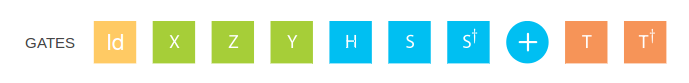
\includegraphics[scale=0.45]{IBMgates.png}
       \caption{\footnotesize{IBM's universal gate set} }
\end{figure}
\vspace{10mm}
\centering{\textbf{How can we implement the $_0^1CR_y(\frac{\pi}{4})$ gate?}}

\end{frame}
}

{
\setbeamertemplate{frame footer}{\tiny{\textsuperscript{1}Nielsen, M. A., \& Chuang, I. L. (2010). Quantum computation and quantum information. Cambridge University Press.\newline \textsuperscript{2}Jat, R. N., \& Ruhela, D. S. (2011). Comparative study of complexity of algorithms for iterative solution of non-linear equations. Journal of International Academy Of Physical Sciences, 15(4).}}
\begin{frame}{Controlled U gate}

\begin{minipage}[t]{.4\textwidth}
	%\vspace{-20mm}
	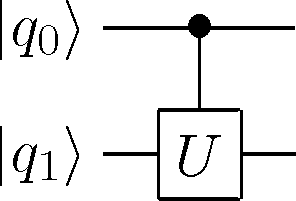
\includegraphics[height=0.5\textwidth]{controlledU.png}
       \captionsetup{justification=raggedright, singlelinecheck=false}
       \captionof{figure}{\footnotesize{Controlled U-gate} }
\end{minipage}%%%%%
\begin{minipage}[t]{.6\textwidth}
%\vspace{-20mm}
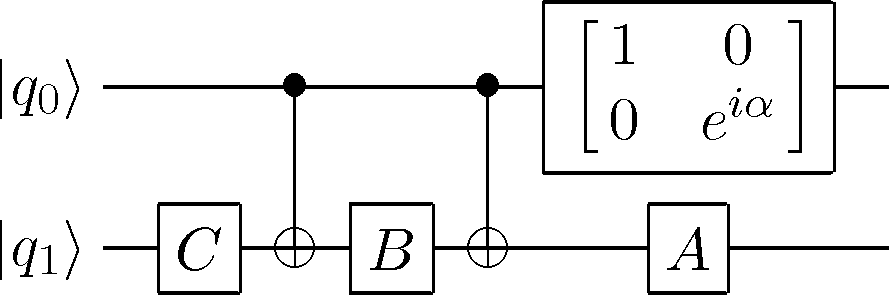
\includegraphics[width=1\textwidth]{controlledUdecomposition.png}
       \captionsetup{justification=raggedright, singlelinecheck=false}
       \captionof{figure}{\footnotesize{Decomposition of a controlled U-gate\textsuperscript{1}} }
\end{minipage}

Choose A,B,C and $\alpha$ s.t.
\begin{equation}
e^{i\alpha}*A*X*B*X*C = U \quad and \quad A*B*C = \mathds{1}
\end{equation}
Need to solve the following equation\textsuperscript{1}
\begin{equation}
U = \begin{pmatrix}
 e^{i(\alpha-\frac{\beta}{2}-\frac{\delta}{2})}\cos{\frac{\gamma}{2}} & -e^{i(\alpha-\frac{\beta}{2}+\frac{\delta}{2})}\sin{\frac{\gamma}{2}} \\ 
e^{i(\alpha+\frac{\beta}{2}-\frac{\delta}{2})}\sin{\frac{\gamma}{2}} & e^{i(\alpha+\frac{\beta}{2}+\frac{\delta}{2})}\cos{\frac{\gamma}{2}}
 \end{pmatrix}
\end{equation}

%calculating a root of a function f(x) with n-digit precision, provided that a good initial approximation is known, is O((\log n) F(n)) where F(n) is the cost of calculating f(x)/f'(x)\, with n-digit precision.

	\metroset{block=fill}
	\begin{alertblock}{Overall algorithmic complexity}
	$\mathcal{O}(\frac{1}{p_{acc}})+\textcolor{red}{\mathcal{O}(k)}$ where $k$ is number of root finding iterations\textsuperscript{2}
	\end{alertblock}
\end{frame}

}

{
\setbeamertemplate{frame footer}{\tiny{\textsuperscript{1}Dawson, C. M., \& Nielsen, M. A. (2005). The Solovay-Kitaev algorithm. arXiv preprint quant-ph/0505030.}}
\begin{frame}{Problems with universal gate sets}

In our case we need to find A, B, C and $\alpha$ for $_0^1CR_y(\frac{\pi}{4})$:

Using a root finding algorithm for non-linear equations we find:

\begin{equation}
\alpha =  \pi; \quad 
\beta = 2\pi;\quad 
\delta = \frac{7}{8}\pi;\quad 
\gamma = 0
\end{equation}
Then,
\begin{align}
A \quad= \quad R_z(\beta)R_y(\frac{\gamma}{2})\quad =& \quad R_z(2\pi) \quad = \quad \textcolor{emerald}{\mathds{1}} \\
B\quad =\quad R_y(-\frac{\gamma}{2})R_z(-\frac{\delta+\beta}{2})\quad =& \quad R_z(-\frac{23}{16}\pi) \quad= \quad \textcolor{red}{???}  \\
C \quad=\quad R_z(\frac{\delta-\beta}{2})\quad =& \quad R_z(-\frac{9}{16}\pi) \quad= \quad \textcolor{red}{???} \\
\begin{pmatrix} 1&0\cr0&e^{i\alpha} \end{pmatrix}\quad=& \quad \begin{pmatrix} 1&0\cr0&e^{i\pi} \end{pmatrix}\quad= \quad \textcolor{emerald}{Z}
\end{align}

\end{frame}
}

{
\setbeamertemplate{frame footer}{\tiny{\textsuperscript{1}Dawson, C. M., \& Nielsen, M. A. (2005). The Solovay-Kitaev algorithm. arXiv preprint quant-ph/0505030.}}
\begin{frame}{The Solovay-Kitaev theorem}

\begin{align}
B\quad =&\quad R_z(-\frac{23}{16}\pi) \quad= \quad \textcolor{red}{???}  \\
C \quad=&\quad R_z(-\frac{9}{16}\pi) \quad= \quad \textcolor{red}{???}
\end{align}

The Solovay-Kitaev theorem guarantees that given a set of single-qubit quantum gates which generates a dense subset of $SU(2)$, then that set is guaranteed to fill $SU(2)$ quickly.\textsuperscript{1}
 
$\rightarrow$ \textcolor{emerald}{\textbf{Hence, given any universal gate set it is possible to obtain good approximations to any desired gate.}}

$\rightarrow$ \textcolor{red}{\textbf{But needs to be computed classically!}}

\end{frame}
}

{
\setbeamertemplate{frame footer}{\tiny{\textsuperscript{1}Booth Jr, J. (2012). Quantum compiler optimizations. arXiv preprint arXiv:1206.3348.}}
\begin{frame}{The Solovay-Kitaev algorithm}

Fowler distance\textsuperscript{1}:
\begin{equation}
dist(U,U_{approx}) = \sqrt{\frac{2-\mid tr(U\cdot U_{approx}^\dagger)\mid}{2}}
\end{equation}

\begin{figure}
    \begin{tikzpicture}[scale=0.8]
\begin{axis}[xlabel={Gate count},ylabel={Fowler distance [$d(U,U_{approx})$]}]

% Graph column 2 versus column 0
\addplot table[x index=1,y index=0,col sep=comma] {datax.dat};
\addlegendentry{$R_z(-\frac{9}{16}\pi)$}% y index+1 since humans count from 1

% Graph column 1 versus column 0    
\addplot table[x index=5,y index=4,col sep=comma] {datax.dat};
\addlegendentry{$R_z(-\frac{23}{16}\pi)$}

\end{axis}
\end{tikzpicture}
  \end{figure}

\end{frame}
}

{
\setbeamertemplate{frame footer}{}
\begin{frame}{The Solovay-Kitaev algorithm}

\begin{minipage}[c]{.8\textwidth}
	%\vspace{-20mm}
	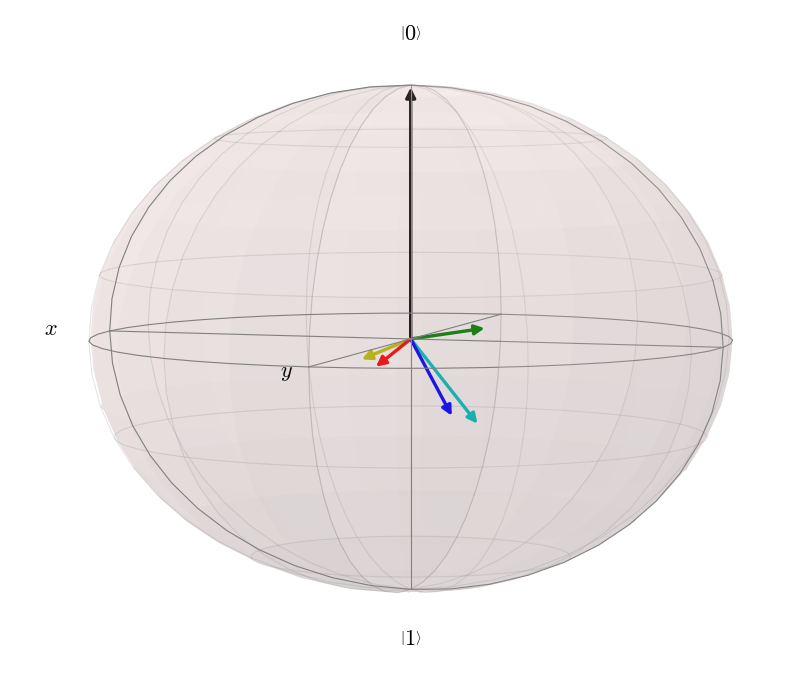
\includegraphics[height=0.8\textwidth]{fowlerdistance.png}
       \captionsetup{justification=raggedright, singlelinecheck=false}
       \captionof{figure}{\footnotesize{Various Fowler distances visualized on Bloch sphere} }
\end{minipage}%%%%%
\begin{minipage}[c]{.2\textwidth}
\scriptsize
\begin{equation}
\textcolor{cyan}{d = 0.22739}
\end{equation}
\begin{equation}
\textcolor{emerald}{d = 0.15165}
\end{equation}
\begin{equation}
\textcolor{blue}{d = 0.10722}
\end{equation}
\begin{equation}
\textcolor{darkyellow}{d = 0.02086}
\end{equation}
\begin{equation}
\textcolor{red}{d = 0.00156}
\end{equation}

\end{minipage}

\end{frame}
}

{
\setbeamertemplate{frame footer}{}
\begin{frame}{The Solovay-Kitaev algorithm}

IBM's quantum computer needs \textbf{130ns for single-qubit gates} and \textbf{500ns for CNOT gates.}

IBM qubit decoherence times:

\SI{49.5}{\micro\second} $\leq T_1 \leq$ \SI{85.3}{\micro\second} "amplitude damping"\\
\SI{56.0}{\micro\second} $\leq T_2 \leq$ \SI{139.7}{\micro\second} "phase damping"
\vspace{6mm}


\begin{table}
    \begin{tabular}{c| c |c |c }
      \toprule
      Approx. Gate & Distance & Gate count & Execution time\\
      \midrule
      $R_z(-\frac{23}{16}\pi)$ & 0.15165 & 25 & \textcolor{emerald}{$\sim$\SI{3}{\micro\second}}\\
       & 0.10722 & 109 & \textcolor{emerald}{$\sim$\SI{14}{\micro\second}}\\
       & 0.02086 & 2997 & \textcolor{red}{$\sim$\SI{390}{\micro\second}}\\
       & 0.01494 & 14721 & \textcolor{red}{$\sim$\SI{1914}{\micro\second}}\\
       & 0.003327 & 74009 & \textcolor{red}{$\sim$\SI{9621}{\micro\second}}\\
       & 0.001578 & 370813 & \textcolor{red}{$\sim$\SI{48206}{\micro\second}}\\
      \bottomrule
    \end{tabular}
    \caption{SK algorithm results}
  \end{table}
 

\end{frame}
}

{
\setbeamertemplate{frame footer}{\tiny{\textsuperscript{1}Dawson, C. M., \& Nielsen, M. A. (2005). The Solovay-Kitaev algorithm. arXiv preprint quant-ph/0505030.}}
\begin{frame}{Adding complexities}

Executing the SK algorithm adds to our overall algorithmic complexity:

\metroset{block=fill}
	\begin{alertblock}{Overall algorithmic complexity}
	$\mathcal{O}(\frac{1}{p_{acc}})+\mathcal{O}(k)+\textcolor{red}{\mathcal{O}(m*log^{2.71}(\frac{m}{\epsilon}))}$ for $\epsilon$-approximations of $m$ gates\textsuperscript{1}
	\end{alertblock}
	
Due to state preparation we went from
\begin{equation}
\mathcal{O}(\frac{1}{p_{acc}})
\end{equation}
suddenly to 
\begin{equation}
\mathcal{O}(m*log^{2.71}(\frac{m}{\epsilon}))
\end{equation}
where $m$ is the number of gates that need approximation to $\epsilon$-accuracy

\end{frame}
}

{
\setbeamertemplate{frame footer}{}
\begin{frame}{Liqui$\ket{}$ simulations}
	
Currently impossible to implement the quantum algorithm on IBM's quantum computer!
$\rightarrow$ can only simulate it with i.e. Liqui$\ket{}$

In Liqui$\ket{}$ we can directly implement the controlled $R_y$ rotation!

%Could you also show what happens if I use approximated gate sequences?	
%Run the command mono Liquid.exe "__BinaryAmplitudeKNN(10000)" in a terminal

\end{frame}
}

\section{Conclusion}

\begin{frame}{Summary}
\begin{itemize}
\item Initial state preparation is non-trivial! (even for very simple examples)
\item In this case, state preparation dominates the overall algorithmic complexity
\item Solovay-Kitaev yields long gate sequences for good approximations
\item Some universal gate sets are only useful when combined with long qubit lifetimes
\item \textbf{Need for better quantum compiling and more general state preparation algorithms!}
\end{itemize}
\end{frame}

\begin{frame}{Taking it further}

\begin{itemize}
\item Complexity analysis of the qubit-based kNN algorithm
\item Classification of gaussian probability distributions
\item Implementing more general state preparation algorithms
\item Waiting for IBM QASM 2.0 ...
\end{itemize}
\end{frame}

\begin{frame}{References}

\footnotesize{Bekkerman, R., Bilenko, M., \& Langford, J. (2011). Scaling up machine learning: Parallel and distributed
approaches. Cambridge University Press.\newline

Booth Jr, J. (2012). Quantum compiler optimizations. arXiv preprint arXiv:1206.3348.

Dawson, C. M., \& Nielsen, M. A. (2005). The Solovay-Kitaev algorithm. arXiv preprint quant-ph/0505030.\newline

IBM. (2016). What is big data? https://www-01.ibm.com/software/data/bigdata/what-is-big
-data.html. (Accessed: 2016-09-08) \newline

Jat, R. N., \& Ruhela, D. S. (2011). Comparative study of complexity of algorithms for iterative solution of non-linear equations. Journal of International Academy Of Physical Sciences, 15(4).\newline

Nielsen, M. A., \& Chuang, I. L. (2010). Quantum computation and quantum information. Cambridge University Press.}
\end{frame}

\begin{frame}[standout]
  Questions?
\end{frame}


\appendix
{
\setbeamertemplate{frame footer}{\vspace{-2mm}\tiny{Chuang I. (2003) MIT Lecture 19: How to Build Your Own Quantum Computer}}
\begin{frame}[fragile]{Backup slide: Qubit decoherence times}

We expect exponential decay:
\begin{equation}
e^{−t/T_i}
\end{equation}

\begin{block}{$T_1$: Longitudinal coherence time (amplitude damping)}

- Prepare $\ket{0}$ state\\
- Apply the X (NOT) gate s.t. qubit is in $\ket{1}$ state\\
- Wait for time $t$\\
- Measure the probability of being in $\ket{1}$ state

\end{block}
\begin{block}{$T_2$: Transversal coherence time (phase damping)}

- Prepare $\ket{0}$ state\\
- Apply Hadamard $\rightarrow \quad \frac{\ket{0}+\ket{1}}{\sqrt{2}}$\\
- Wait for time $t$\\
- Apply Hadamard again\\
- Measure the probability of being in $\ket{0}$ state\\

We expect this probability to go to 0.5 $\rightarrow$ qubit lost quantum behaviour
\end{block}

\end{frame}
}
{
\setbeamertemplate{frame footer}{\tiny{\textsuperscript{1}Li, Z., Liu, X., Xu, N., \& Du, J. (2015). Experimental realization of a quantum support vector machine. Physical Review Letters, 114 (14), 1–5. doi: 10.1103/PhysRevLett.114.140504 \newline\textsuperscript{2}Cai, X. D., Wu, D., Su, Z. E., Chen, M. C., Wang, X. L., Li, L., . . . Pan, J. W. (2015). Entanglement-
based machine learning on a quantum computer. Physical Review Letters, 114 (11), 1–5. doi:10.1103/PhysRevLett.114.110504 \newline\textsuperscript{3}Ristè, D., da Silva, M. P., Ryan, C. A., Cross, A. W., Smolin, J. A., Gambetta, J. M., . . . Johnson,
B. R. (2015). Demonstration of quantum advantage in machine learning. arXiv:1512.06069 , 1–12.
Retrieved from http://arxiv.org/abs/1512.06069 }}
\begin{frame}[fragile]{Backup Slide II: Experimental realizations}


Only few experimental verifications of QML algorithms:

- Li, Liu, Xu, and Du (2015) successfully distinguished a handwritten six from a nine using a
quantum support vector machine on a four-qubit nuclear magnetic resonance test bench\textsuperscript{1}

- Cai et al. (2015) were first to experimentally demonstrate quantum machine learning on a photonic QC and showed that the distance between two vectors and their inner product can indeed be computed quantum
mechanically\textsuperscript{2}

- Ristè et al. (2015) solved a learning parity problem with five superconducting qubits and found that a quantum advantage can already be observed in non error-corrected systems\textsuperscript{3}


%Explain the experimental results that have been shown so far. Outline problems with non-error corrected qubits, gate times and small qubit numbers.

%> only proof-of-concept so far
%little is known about full procedure from crude data to final classification

\end{frame}
}

{
\setbeamertemplate{frame footer}{}
\begin{frame}[fragile]{Machine Learning}
   
Machine learning can be subdivided into three major fields.

\metroset{block=fill}

\begin{alertblock}{Supervised ML}
- Based on \emph{input} and \emph{output} data\\
\centering{
"I know how to classify this data but I need the algorithm to do the computations for me."}
\end{alertblock}

\begin{exampleblock}{Unsupervised ML}
- Based on \emph{input} data only\\
\centering{
"I have no clue how to classify this data, can the algorithm create a classifier for me?"}
\end{exampleblock}

\begin{block}{Reinforcement learning}
- Based on \emph{input} data only\\
\centering{
"I have no clue how to classify this data, can the algorithm classify this data and I'll give it a reward if it's correct or I'll punish it if it's not."}
\end{block}

\end{frame}
}

{
\setbeamertemplate{frame footer}{}
\begin{frame}[fragile]{Machine Learning}
   
Machine learning can be subdivided into three major fields.

\metroset{block=fill}

\begin{alertblock}{Supervised ML}
- Based on \emph{input} and \emph{output} data\\
\centering{
"I know how to classify this data but I need the algorithm to do the computations for me."}
\end{alertblock}

\begin{exampleblock}{\textcolor{gray}{Unsupervised ML}}
\color{gray}
- Based on \emph{input} data only\\
\centering{
"I have no clue how to classify this data, can the algorithm create a classifier for me?"}
\end{exampleblock}

\begin{block}{\textcolor{gray}{Reinforcement learning}}
\color{gray}
- Based on \emph{input} data only\\
\centering{
"I have no clue how to classify this data, can the algorithm classify this data and I'll give it a reward if it's correct or I'll punish it if it's not."}
\end{block}

\end{frame}
}

{
\setbeamertemplate{frame footer}{}
\begin{frame}{Liqui$\ket{}$ simulations: Taking it further}

\begin{figure}
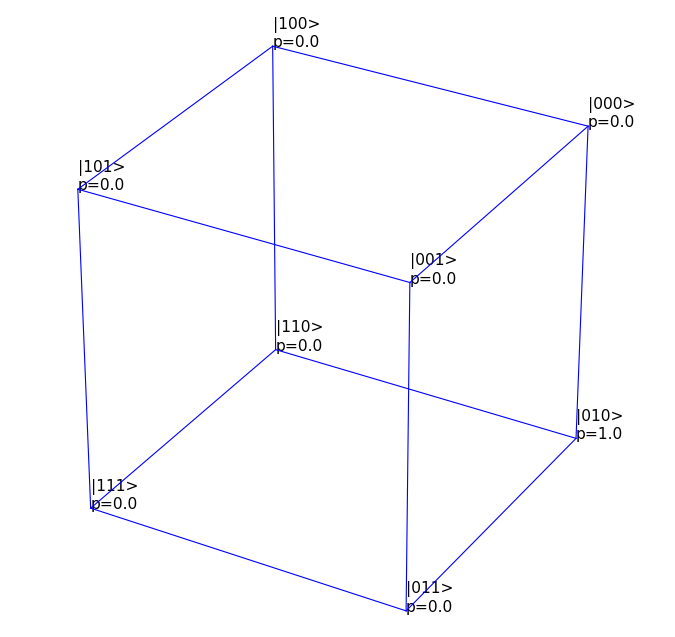
\includegraphics[scale=0.35]{cube_notdiffused.png}
       \caption{\footnotesize{Representation of hamming distance on 3D cube} }
\end{figure}
\end{frame}
}

{
\setbeamertemplate{frame footer}{}
\begin{frame}{Liqui$\ket{}$ simulations: Taking it further}

Applying the following matrix
\begin{equation}
\begin{pmatrix}
 \sqrt{\delta} & 1-\sqrt{\delta} \\ 
 1-\sqrt{\delta} & -\sqrt{\delta}
 \end{pmatrix}
\end{equation}
to all qubits in the data register leads to a gaussian distribution over the "Hamming distance" cube:

\begin{figure}
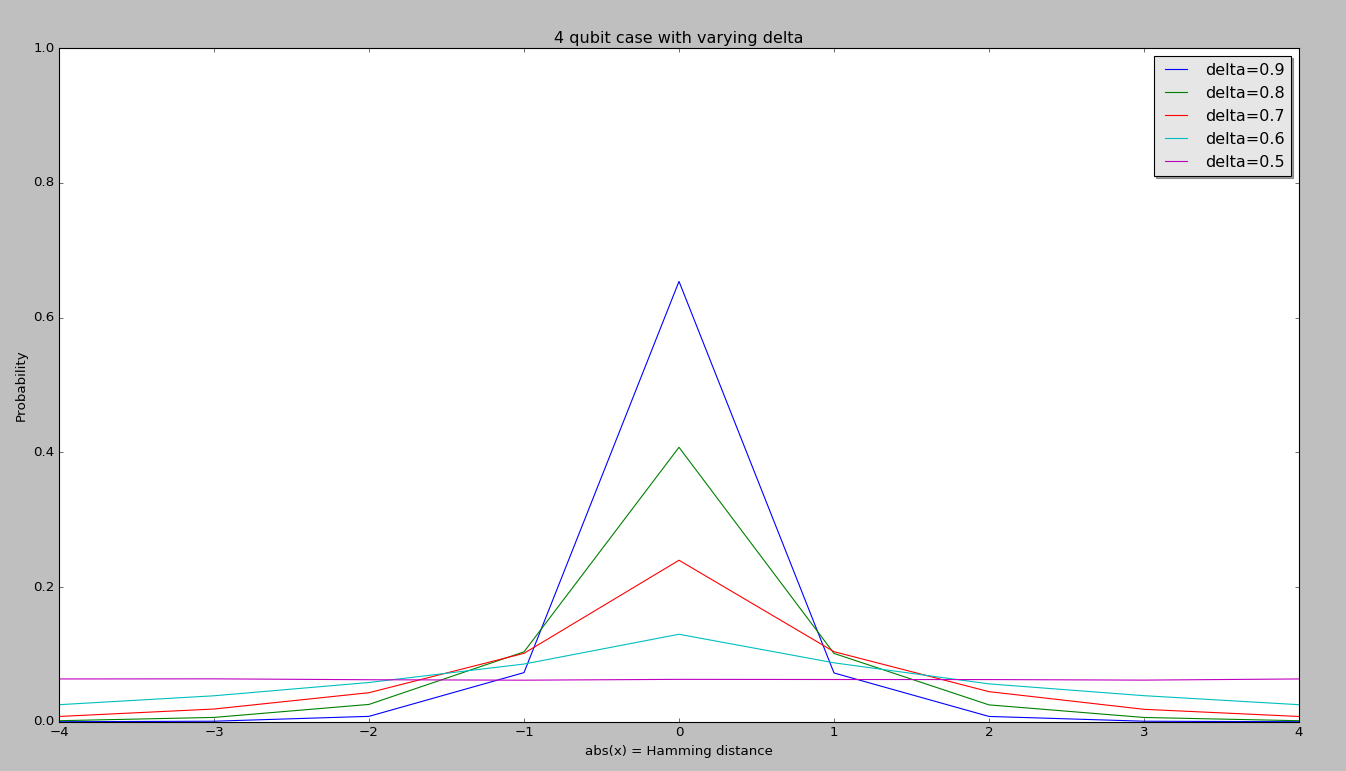
\includegraphics[scale=0.2]{4qubitdiffusion.png}
       \caption{\footnotesize{Gaussian diffusion of a quantum state} }
\end{figure}

\end{frame}
}

{
\setbeamertemplate{frame footer}{}
\begin{frame}{Liqui$\ket{}$ simulations: Taking it further}

\begin{figure}
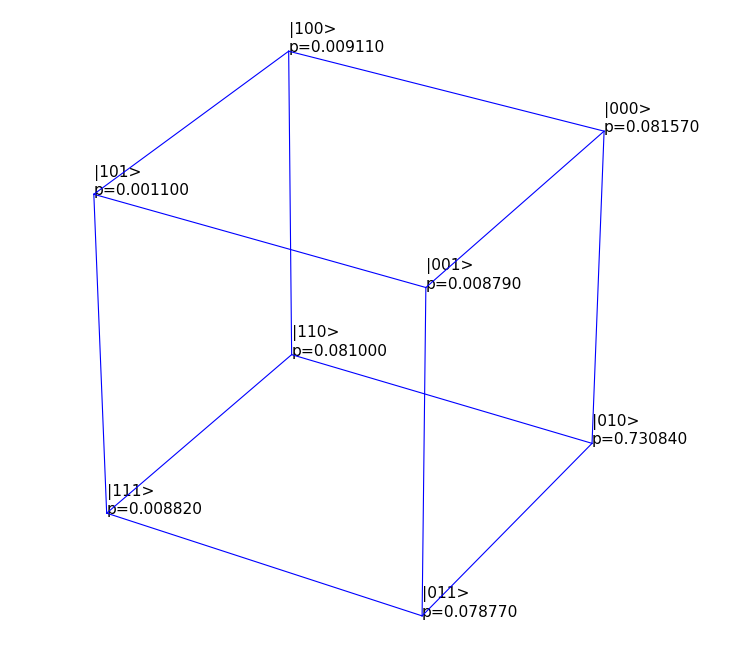
\includegraphics[scale=0.33]{cube_diffused.png}
       \caption{\footnotesize{Representation of gaussian diffusion on 3D cube} }
\end{figure}
\end{frame}
}

{
\setbeamertemplate{frame footer}{}
\begin{frame}{Liqui$\ket{}$ simulations: Taking it further}

\begin{figure}
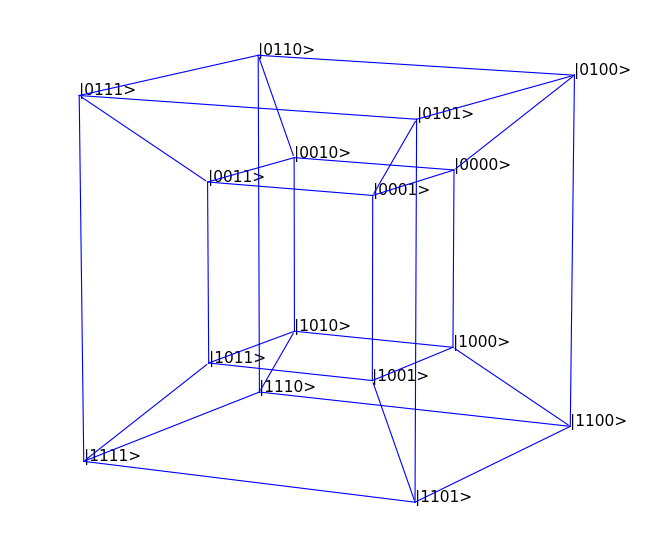
\includegraphics[scale=0.33]{4d_hypercube.png}
       \caption{\footnotesize{Representation of gaussian diffusion on 3D cube} }
\end{figure}
\end{frame}
}

\begin{frame}[allowframebreaks]{Backup slide II}

  \bibliography{demo}
  \bibliographystyle{abbrv}

\end{frame}

\section{Qubit-based kNN quantum algorithm}

{
\setbeamertemplate{frame footer}{References go here}
\begin{frame}[fragile]{Typography}
      \begin{verbatim}The theme provides sensible defaults to
\emph{emphasize} text, \alert{accent} parts
or show \textbf{bold} results.\end{verbatim}

  \begin{center}becomes\end{center}

  The theme provides sensible defaults to \emph{emphasize} text,
  \alert{accent} parts or show \textbf{bold} results.
\end{frame}
}

{
\setbeamertemplate{frame footer}{References go here}
\begin{frame}{Font feature test}
  \begin{itemize}
    \item Regular
    \item \textit{Italic}
    \item \textsc{SmallCaps}
    \item \textbf{Bold}
    \item \textbf{\textit{Bold Italic}}
    \item \textbf{\textsc{Bold SmallCaps}}
    \item \texttt{Monospace}
    \item \texttt{\textit{Monospace Italic}}
    \item \texttt{\textbf{Monospace Bold}}
    \item \texttt{\textbf{\textit{Monospace Bold Italic}}}
  \end{itemize}
\end{frame}
}

\begin{frame}{Lists}
  \begin{columns}[T,onlytextwidth]
    \column{0.33\textwidth}
      Items
      \begin{itemize}
        \item Milk \item Eggs \item Potatos
      \end{itemize}

    \column{0.33\textwidth}
      Enumerations
      \begin{enumerate}
        \item First, \item Second and \item Last.
      \end{enumerate}

    \column{0.33\textwidth}
      Descriptions
      \begin{description}
        \item[PowerPoint] Meeh. \item[Beamer] Yeeeha.
      \end{description}
  \end{columns}
\end{frame}
\begin{frame}{Animation}
  \begin{itemize}[<+- | alert@+>]
    \item \alert<4>{This is\only<4>{ really} important}
    \item Now this
    \item And now this
  \end{itemize}
\end{frame}
\begin{frame}{Figures}
  \begin{figure}
    \newcounter{density}
    \setcounter{density}{20}
    \begin{tikzpicture}
      \def\couleur{alerted text.fg}
      \path[coordinate] (0,0)  coordinate(A)
                  ++( 90:5cm) coordinate(B)
                  ++(0:5cm) coordinate(C)
                  ++(-90:5cm) coordinate(D);
      \draw[fill=\couleur!\thedensity] (A) -- (B) -- (C) --(D) -- cycle;
      \foreach \x in {1,...,40}{%
          \pgfmathsetcounter{density}{\thedensity+20}
          \setcounter{density}{\thedensity}
          \path[coordinate] coordinate(X) at (A){};
          \path[coordinate] (A) -- (B) coordinate[pos=.10](A)
                              -- (C) coordinate[pos=.10](B)
                              -- (D) coordinate[pos=.10](C)
                              -- (X) coordinate[pos=.10](D);
          \draw[fill=\couleur!\thedensity] (A)--(B)--(C)-- (D) -- cycle;
      }
    \end{tikzpicture}
    \caption{Rotated square from
    \href{http://www.texample.net/tikz/examples/rotated-polygons/}{texample.net}.}
  \end{figure}
\end{frame}
\begin{frame}{Tables}
  \begin{table}
    \caption{Largest cities in the world (source: Wikipedia)}
    \begin{tabular}{lr}
      \toprule
      City & Population\\
      \midrule
      Mexico City & 20,116,842\\
      Shanghai & 19,210,000\\
      Peking & 15,796,450\\
      Istanbul & 14,160,467\\
      \bottomrule
    \end{tabular}
  \end{table}
\end{frame}
\begin{frame}{Blocks}
  Three different block environments are pre-defined and may be styled with an
  optional background color.

  \begin{columns}[T,onlytextwidth]
    \column{0.5\textwidth}
      \begin{block}{Default}
        Block content.
      \end{block}

      \begin{alertblock}{Alert}
        Block content.
      \end{alertblock}

      \begin{exampleblock}{Example}
        Block content.
      \end{exampleblock}

    \column{0.5\textwidth}

      \metroset{block=fill}

      \begin{block}{Default}
        Block content.
      \end{block}

      \begin{alertblock}{Alert}
        Block content.
      \end{alertblock}

      \begin{exampleblock}{Example}
        Block content.
      \end{exampleblock}

  \end{columns}
\end{frame}
\begin{frame}{Math}
  \begin{equation*}
    e = \lim_{n\to \infty} \left(1 + \frac{1}{n}\right)^n
  \end{equation*}
\end{frame}
\begin{frame}{Line plots}
  \begin{figure}
    \begin{tikzpicture}
      \begin{axis}[
        mlineplot,
        width=0.9\textwidth,
        height=6cm,
      ]

        \addplot {sin(deg(x))};
        \addplot+[samples=100] {sin(deg(2*x))};

      \end{axis}
    \end{tikzpicture}
  \end{figure}
\end{frame}
\begin{frame}{Bar charts}
  \begin{figure}
    \begin{tikzpicture}
      \begin{axis}[
        mbarplot,
        xlabel={Foo},
        ylabel={Bar},
        width=0.9\textwidth,
        height=6cm,
      ]

      \addplot plot coordinates {(1, 20) (2, 25) (3, 22.4) (4, 12.4)};
      \addplot plot coordinates {(1, 18) (2, 24) (3, 23.5) (4, 13.2)};
      \addplot plot coordinates {(1, 10) (2, 19) (3, 25) (4, 15.2)};

      \legend{lorem, ipsum, dolor}

      \end{axis}
    \end{tikzpicture}
  \end{figure}
\end{frame}
\begin{frame}{Quotes}
  \begin{quote}
    Veni, Vidi, Vici
  \end{quote}
\end{frame}


\end{document}
